\documentclass[journal]{IEEEtran}
\usepackage[T1]{fontenc}
\usepackage{amsmath,amssymb,graphicx,booktabs,array,url,balance,textcomp}
\newcolumntype{L}[1]{>{\raggedright\arraybackslash}p{#1}}
\usepackage[hidelinks]{hyperref}
\graphicspath{{figs/}}
\newcommand{\du}{\Delta u_{\mathrm{c}}}
% GENERATED by scripts/final_closure_manuscript_tables.py -- do not edit
% every number below is read from research/final_closure/
\newcommand{\NballMatched}{54}
\newcommand{\RloopZone}{2.262}
\newcommand{\RloopZtwo}{1.540}
\newcommand{\PlossZone}{149.06}
\newcommand{\PlossZtwo}{148.04}
\newcommand{\TmaxZone}{122.32}
\newcommand{\TmaxZtwo}{124.60}
\newcommand{\TdieZone}{90.06}
\newcommand{\TdieZtwo}{90.00}
\newcommand{\WarpZone}{27.90}
\newcommand{\WarpZtwo}{68.81}
\newcommand{\DuZone}{2.394}
\newcommand{\DuZtwo}{3.090}
\newcommand{\WarpRatio}{2.47}
\newcommand{\DuRatio}{1.29}
\newcommand{\EpsZone}{$6.284\times10^{-3}$}
\newcommand{\EpsZtwo}{$7.241\times10^{-3}$}
\newcommand{\EpsRatio}{1.15}
\newcommand{\EtIters}{7}
\newcommand{\ErrTsvBulk}{1.15}
\newcommand{\ErrTsvKz}{0.71}
\newcommand{\ErrTsvKx}{0.25}
\newcommand{\ErrRdlKx}{3.69}
\newcommand{\ErrRdlKz}{12.49}
\newcommand{\ErrPkgRdlZone}{0.079}
\newcommand{\ErrPkgRdlZtwo}{0.11}
\newcommand{\ErrThermAedtZone}{0.14}
\newcommand{\ErrThermAedtZtwo}{0.11}
\newcommand{\ErrThermMooseZone}{0.16}
\newcommand{\ErrThermMooseZtwo}{0.12}
\newcommand{\ErrMechClosed}{0.43}
\newcommand{\ErrMechAedt}{0.014}
\newcommand{\ErrSolverIter}{0.010}
\newcommand{\ErrCoolingIcepak}{16.48}
\newcommand{\SpeedTsvBulk}{15964476}
\newcommand{\SpeedTsvKz}{50373947}
\newcommand{\SpeedTsvKx}{45013210}
\newcommand{\SpeedRdlKx}{54299699}
\newcommand{\SpeedRdlKz}{26039527}
\newcommand{\SpeedPkgRdlZone}{3.47}
\newcommand{\SpeedPkgRdlZtwo}{2.49}
\newcommand{\SpeedThermAedtZone}{2.19}
\newcommand{\SpeedThermAedtZtwo}{3.03}
\newcommand{\SpeedThermMooseZone}{0.43}
\newcommand{\SpeedThermMooseZtwo}{0.66}
\newcommand{\SpeedMechClosed}{n/a}
\newcommand{\SpeedMechAedt}{3.99}
\newcommand{\SpeedSolverIter}{n/a}
\newcommand{\SpeedCoolingIcepak}{76500623}
\newcommand{\EnergyTol}{1e-06}
\newcommand{\MeshTol}{2}
\newcommand{\MeshWorstProd}{1.35}
\newcommand{\MeshBaseTmaxZone}{4.91}
\newcommand{\MeshBaseTmaxZtwo}{2.67}
\newcommand{\EtWallZone}{2118}
\newcommand{\EtWallZtwo}{2079}
\newcommand{\MechWallZone}{1430}
\newcommand{\MechWallZtwo}{2664}
\newcommand{\NjointZone}{1369}
\newcommand{\NjointZtwo}{528}
\newcommand{\MeshBoundSentence}{}
\newcommand{\LocalMeshPhrase}{mesh-refined with a quantified discretisation bound}
\newcommand{\LocalLevel}{L3}
\newcommand{\EpsUZone}{2.01}
\newcommand{\EpsUZtwo}{29.22}
\newcommand{\UtimeMax}{0.027}
\newcommand{\UcycMax}{0.80}
\newcommand{\LocalNconverged}{2}
\newcommand{\LocalNcases}{4}
\newcommand{\LocalAccepted}{accepted}
\newcommand{\NgatesB}{31}
\newcommand{\NbOne}{29}
\newcommand{\NbTwo}{2}
\newcommand{\NbThree}{0}
\newcommand{\BoneResolved}{29}
\newcommand{\RstarSzero}{1.77}
\newcommand{\PfeedRstarSzero}{1.01}
\newcommand{\AdvZeroFeedSzero}{1.02}
\newcommand{\IrmsSzero}{23.9}
\newcommand{\PfeedPerMohmSzero}{0.572}
\newcommand{\EffRstarSzero}{87.03}
\newcommand{\RstarSone}{3.76}
\newcommand{\PfeedRstarSone}{36.75}
\newcommand{\AdvZeroFeedSone}{36.75}
\newcommand{\IrmsSone}{95.8}
\newcommand{\PfeedPerMohmSone}{9.184}
\newcommand{\EffRstarSone}{84.26}
\newcommand{\RstarStwo}{n/a}
\newcommand{\PfeedRstarStwo}{n/a}
\newcommand{\AdvZeroFeedStwo}{159.87}
\newcommand{\IrmsStwo}{166.6}
\newcommand{\PfeedPerMohmStwo}{27.758}
\newcommand{\EffRstarStwo}{n/a}
\newcommand{\FeedSweepLo}{0.01}
\newcommand{\FeedSweepHi}{100}
\newcommand{\FeedSweepN}{241}
\newcommand{\AttachH}{30}
\newcommand{\AttachCu}{14}
\newcommand{\AttachCap}{16}
\newcommand{\AttachD}{15}
\newcommand{\AttachPitch}{30}
\newcommand{\AttachNbump}{3042}
\newcommand{\AttachAreaPct}{19.6}
\newcommand{\AttachKz}{19.1}
\newcommand{\AttachKxy}{0.89}
\newcommand{\AttachEgpa}{8}
\newcommand{\AttachCte}{30}
\newcommand{\AttachPw}{0.234}
\newcommand{\TsvPwZtwo}{0.555}
\newcommand{\CutoutMM}{23.36}
\newcommand{\ClearanceMM}{1.0}
\newcommand{\FillExtentMM}{10.68}
\newcommand{\NsitesZone}{1369}
\newcommand{\NsitesZtwo}{528}
\newcommand{\SubZtwoUM}{300}
\newcommand{\IcepakFactor}{1.165}
\newcommand{\PlossCtrl}{149.30}
\newcommand{\TmaxCtrl}{124.84}
\newcommand{\WarpCtrl}{69.01}
\newcommand{\DuCtrl}{3.113}
\newcommand{\CtrlPkgHV}{1.171}
\newcommand{\CtrlMinusZtwo}{1.26}
\newcommand{\AttDenseD}{15}
\newcommand{\AttDenseP}{30}
\newcommand{\AttDenseNvdd}{3042}
\newcommand{\AttDenseNgnd}{3042}
\newcommand{\AttDenseNaxis}{78}
\newcommand{\AttDenseFpct}{19.2}
\newcommand{\AttDensePw}{0.238}
\newcommand{\AttDenseRbump}{17.42}
\newcommand{\AttDenseConstrPct}{1.3}
\newcommand{\AttDenseImA}{6.8}
\newcommand{\AttDenseJkacm}{3.83}
\newcommand{\AttDenseLambda}{0.12}
\newcommand{\AttDenseKz}{18.7}
\newcommand{\AttDenseKxy}{0.88}
\newcommand{\AttDenseEB}{19.6}
\newcommand{\ErrAttDenseKz}{+0.5}
\newcommand{\ErrAttDenseKxy}{+0.4}
\newcommand{\AttDensePzTwo}{148.05}
\newcommand{\AttDenseFracPct}{0.16}
\newcommand{\AttSparseD}{30}
\newcommand{\AttSparseP}{80}
\newcommand{\AttSparseNvdd}{421}
\newcommand{\AttSparseNgnd}{420}
\newcommand{\AttSparseNaxis}{29}
\newcommand{\AttSparseFpct}{10.6}
\newcommand{\AttSparsePw}{0.465}
\newcommand{\AttSparseRbump}{4.71}
\newcommand{\AttSparseConstrPct}{8.9}
\newcommand{\AttSparseImA}{48.9}
\newcommand{\AttSparseJkacm}{6.91}
\newcommand{\AttSparseLambda}{0.17}
\newcommand{\AttSparseKz}{10.6}
\newcommand{\AttSparseKxy}{0.74}
\newcommand{\AttSparseEB}{14.3}
\newcommand{\ErrAttSparseKz}{+1.3}
\newcommand{\ErrAttSparseKxy}{+0.2}
\newcommand{\AttSparsePzTwo}{148.72}
\newcommand{\AttSparseFracPct}{0.31}
\newcommand{\AttDeltaPetm}{0.66}
\newcommand{\AttDeltaPatt}{0.23}
\newcommand{\AttDeltaPconv}{0.43}
\newcommand{\AttDeltaTconv}{0.75}
\newcommand{\AttPenBlock}{0.23}
\newcommand{\AttPenNet}{0.27}
\newcommand{\AttNetFactor}{1.21}
\newcommand{\AttPeakMean}{1.65}
\newcommand{\AttFstarPct}{17.4}
\newcommand{\AttPstar}{31.7}
\newcommand{\AttFstarNetPct}{17.5}
\newcommand{\AttPstarNet}{31.6}
\newcommand{\RstarDenseSzero}{1.74}
\newcommand{\RstarSparseSzero}{0.58}


\begin{document}

\title{Electrothermal--Mechanical Closure of Distributed Vertical Power Delivery: Architecture Preference Is Conditional on the Coupled Implementation}

\author{Mohamed~Gharib and Inna~Partin-Vaisband% author list to be confirmed
\thanks{Manuscript prepared September 2026.}}

\maketitle

\begin{abstract}
Kilowatt-scale power delivery is package-limited. A hierarchical
electrothermal--mechanical framework for distributed vertical power delivery carries converter
synthesis into an explicit physical package---conductor-level ledger, tier-resolved heat map,
converged electrothermal fixed point, thermoelastic solution, all-site critical-joint search and
viscoplastic solder submodel---each checked against a matched reference. It is applied to a 1\,kW, 48\,V-to-1\,V, 49-cell
regulator system in two physically closed architectures: a regulator embedded between
substrate and die (Z1), fed through the ball-grid array, and a backside regulator in a board
opening (Z2), fed directly at 48\,V so that only 1\,V crosses the substrate. Physically closing the architectures reveals that no architecture can be ranked independently of its neighboring design decisions: the external feed resistance decides the platform-level electrical preference, through-silicon-via provisioning can reverse the package-internal one, the regulator-to-substrate attach density can change it, cooling and the out-of-cell construction can reverse the mechanical preference, and local construction determines the solder response.
Inside the declared package boundary the backside regulator dissipates \PlossZtwo\,W against \PlossZone\,W in the headline scenario; its external feed lies outside that boundary, so the platform-level preference is conditional: the complete 48\,V feed loop must stay below \RstarSzero\,m$\Omega$. The embedded architecture has the lower die warpage and joint displacement driver; the peak temperature ordering reverses between scenarios; the local solder response difference lies within the measured discretisation uncertainty.
The overall-ratio pulse drives the embedded joints to the solder melting onset; no comparison is drawn there. No absolute life, qualification or commercial speedup is claimed.
\end{abstract}

\begin{IEEEkeywords}
Distributed vertical power delivery, electrothermal--mechanical co-design, package power
delivery network, local inelastic response, solder fatigue response, physical realizability,
through-substrate vias, heterogeneous integration.
\end{IEEEkeywords}
\section{Introduction}\label{sec:intro}

\IEEEPARstart{P}{ower} demand in high-performance computing is projected to reach one to
two kilowatts per compute die, delivered at core voltages near one
volt~\cite{Krishnakumar2026DVPD,Ramin_VPD}. At that operating point the delivery network,
rather than the regulator, limits the achievable efficiency. For a 1\,kW load at 1\,V the
total current approaches one kiloampere, and direct lateral delivery of that current in the
evaluated package stack is prohibitively lossy: the $I^{2}R$ dissipation of a 1\,V rail
traversing even a few millimetres of package metal becomes comparable with the load itself.
Higher-voltage or vertical distribution is therefore required.

Vertical power delivery (VPD) addresses this by converting in or near the package beneath
the load, removing the long board-to-package lateral path~\cite{Sriharini_ECTC_24}. Converting
vertically is not by itself sufficient, however: with a single lumped regulator the
post-conversion low-voltage, high-current rail must still traverse the package or interposer
redistribution layers to reach spatially separated points of load, a distance reported as up
to a quarter of the system perimeter~\cite{Krishnakumar2026DVPD}. Distributed vertical power
delivery (DVPD) answers \emph{that} by partitioning conversion into many regulator cells
placed laterally beneath or around their corresponding load regions, so that high-voltage,
low-current power is distributed laterally first and the residual high-current rail travels
micrometres rather than millimetres, with the per-cell output current scaling as
$I_{\mathrm{o}}/M$~\cite{Krishnakumar2026DVPD,Sriharini_ECTC_24,
VPD_transactions_on_power_electronics_new,
ISCAS2024DVPD,vertical_stacking_2025_TRansactions_power_electronics}. DVPD is therefore a
distributed form of vertical power delivery, and the quantity that distinguishes the two is
the low-voltage lateral path that survives conversion.
Design frameworks for DVPD have advanced considerably. Converter synthesis, interconnect
allocation, floorplanning and thermal feasibility are now co-optimised within a single
flow~\cite{Krishnakumar2026DVPD}; effective models for vertical routing over C4 bumps,
through-silicon vias and micro-bumps have been formulated~\cite{Sriharini_ECTC_24}; and
package-embedded passive components have been demonstrated at the densities such
architectures require~\cite{rasheedi2024embedded,multi-layer_inductor}. Electrothermal
co-optimization of the power distribution network itself, including a manufacturing-cost
objective, has been reported for 2.5-D systems~\cite{Wang2025TTSV}.

What these frameworks share is a domain boundary. Electrical and thermal quantities are
co-optimised; package mechanics and interconnect manufacturability are evaluated afterwards,
on a geometry the electrical optimisation has already fixed. The separation is convenient
but not obviously safe, because the converter-design variables that the electrical
optimisation selects are the variables that set the mechanical and packaging problem. The
number of regulator cells fixes the footprint each cell may occupy. The device and passive
selections fix the component heights and therefore the substrate thickness. The partition of
components across tiers fixes which rail crosses which vertical interconnect, and hence both
the interconnect loss and the depth at which heat is deposited. The resulting stack of
dissimilar materials fixes the coefficient-of-thermal-expansion mismatch that drives solder
deformation. A design that is electrically and thermally attractive may therefore be
mechanically distinct, or physically unbuildable, for reasons the electrical model cannot
express.

Thermomechanical analysis of packages is itself mature, and placement studies accounting for
warpage and solder fatigue are established~\cite{Syed2004,Schubert2003}. What is missing is
the connection: a formulation in which converter-synthesis outputs are propagated into an
explicit package stack, and in which the electrical, thermal, mechanical and realizability
questions are asked of the same geometry. Establishing that connection, and reporting what
it changes, is the subject of this paper.

% BEGIN final-lineage:intro-claim
Recent DVPD work has established design considerations for the distributed
regulators themselves~\cite{ISCAS2024DVPD}, buck-derived vertical delivery~\cite{Sriharini_ECTC_24},
a comprehensive electrical and thermal design framework~\cite{Krishnakumar2026DVPD},
self-consistent electrothermal models with embedded microfluidic
cooling~\cite{Choi2024ITherm,Choi2025SelfConsistent}, and system perspectives on the path from
lateral to vertical delivery~\cite{VPD2023Architectures,Ye2026TenKiloAmp,Swaminathan2026IVPDReview}.
The present paper does not re-derive that design flow. Its subject is narrower: what happens to
an architecture comparison when both alternatives are closed as physical packages---every
conductor owned, every interface explicit, every heat source in its own tier---and the
electrical, thermal and mechanical questions are asked of the same geometry. Physically closing the architectures reveals that no architecture can be ranked independently of its neighboring design decisions: the external feed resistance decides the platform-level electrical preference, through-silicon-via provisioning can reverse the package-internal one, the regulator-to-substrate attach density can change it, cooling and the out-of-cell construction can reverse the mechanical preference, and local construction determines the solder response. A coupled electrothermal--mechanical framework is therefore required to make an architecture-level decision.
% END final-lineage:intro-claim
The following contributions are made.

\begin{enumerate}
\item A geometry- and architecture-aware electrothermal--mechanical framework for DVPD is
presented, in which converter-synthesis outputs---device selection, branch count, switching
frequency, component heights and cell footprint---are propagated into an explicit package
stack rather than into a lumped loss budget (Sections~\ref{sec:elec}--\ref{sec:thermech}).

\item A rail-aware power-delivery network model is developed in which each vertical segment
carries the rail actually assigned to it, and in which interconnect resistance is derived
from via geometry, allocation policy, temperature-dependent resistivity and the land
geometry of the connected device, rather than from a lumped crowding factor
(Section~\ref{sec:elec}).

\item Physical realizability is coupled to the same geometry that produces the electrical
and thermal results. The number of vertical via levels is derived from the conductor-plane
sequence of the build-up stack rather than from its material-layer count, and a
framework provisioning state is reported separately from a manufacturing-qualification
state (Sections~\ref{sec:elec}-E and~\ref{sec:arch}).

\item A mechanical formulation is developed that progresses from global package deformation
through a corner-joint displacement driver to a displacement-driven local solder inelastic-response submodel (\LocalMeshPhrase), and the two are reported as
separate quantities: the driver is a displacement in micrometres, the response a
dimensionless strain increment per stabilised cycle. The terminology ladder from response
through damage to life is kept explicit (Section~\ref{sec:thermech}).

\item Six positions taken in the prior DVPD literature are reproduced within the framework
and tested. Two are reproduced, one is found to be rail-dependent, one reverses with the
assembly state, one is invalidated by physical realizability, and one---peak temperature as
a reliability ranking---is shown to be non-equivalent to the local mechanical response
(Section~\ref{sec:compare}).
% BEGIN final-lineage:contrib
\item A voltage-fed, return-inclusive package power-delivery network is solved on a
finite-volume grid whose faces are aligned with every regulator terminal, which converges
where a uniform grid cannot; the ball-grid-array count is treated as a solved integer design
variable rather than sized from an equal-sharing assumption that the network disproves
(Section~\ref{sec:pdnclosure}).

\item The backside architecture is closed as a physical package: its 48\,V input enters the
regulator directly through the board opening, only 1\,V crosses the substrate through an
explicit converter-to-substrate attach, and the converter clears the opening sidewall. The
unsourced external feed is swept rather than assumed, which turns it into a design
requirement---a maximum loop resistance---instead of an invented connector
(Sections~\ref{sec:physarch} and~\ref{sec:directfeed}).

\item Every reduced model is checked stage by stage against a matched reference on the same
problem and machine---commercial and open-source finite elements, closed forms and a conjugate
fluid-dynamics solution---and model-specific errors and runtimes are reported in place of a
single framework accuracy (Section~\ref{sec:matched}).

\item Every ordering-relevant input without a single defensible value is run on the production
mesh and judged by the same uncertainty-aware rule as the production pair; the orderings that
reverse are reported as a central result, not as a caveat (Section~\ref{sec:classb}).
% END final-lineage:contrib
\end{enumerate}

\section{DVPD System and Physical Architectures}\label{sec:system}

\subsection{System specification}
\begin{table}[!t]
\caption{System specification and synthesised converter design point.}
\label{tab:spec}
\centering
\footnotesize
\setlength{\tabcolsep}{2.5pt}
\begin{tabular}{@{}llc@{}}
\toprule
Quantity & Value & Source \\
\midrule
\multicolumn{3}{@{}l}{\emph{System}}\\
Load power / voltage        & 1\,kW / 1\,V              & specification \\
Platform rail               & 48\,V                     & specification \\
Compute die                 & $22.36\times22.36$\,mm    & specification \\
Regulator cells $M$         & 49                        & synthesis \\
Current per cell            & $20.408$\,A               & derived \\
Cell footprint              & $5.61$\,mm$^{2}$          & synthesis \\
Target current density      & $3.5$\,A\,mm$^{-2}$       & specification \\
\midrule
\multicolumn{3}{@{}l}{\emph{Converter}}\\
Architecture $N/K/K_{A}$    & $3/3/2$                   & synthesis \\
Topology                    & 3:1 SC + two-phase buck, & \cite{DSCH,DPMIH44} \\
                             & $K{=}3$ inductor branches &  \\
Duty cycle $D$              & $0.0625$                  & synthesis \\
Switching frequency         & $805.17$\,kHz             & synthesis \\
High-side device            & EPC2014C, $16$\,m$\Omega$, $1.87$\,mm$^{2}$ & \cite{EPC2014C} \\
Low-side device             & EPC2057, $8.5$\,m$\Omega$, $1.80$\,mm$^{2}$ & \cite{EPC2057} \\
Inductor                    & $250$\,nH, $1.6$\,m$\Omega$, $500$\,\textmu m & \cite{rasheedi2024embedded} \\
Flying / output cap.\       & $10$\,\textmu F, $2.5$\,m$\Omega$, $2.0$\,mm$^{2}$ & datasheet \\
Loss per cell at $25\,^{\circ}$C & $1.866$\,W           & loss model \\
\midrule
\multicolumn{3}{@{}l}{\emph{Package and cooling}}\\
Substrate thickness, Z1 / Z2 & $1.30$ / $0.30$\,mm      & architecture \\
Converter component stack    & $1953$\,\textmu m\,/\,$1921$\,\textmu m & components$^{\dagger}$ \\
Embedded in Z1 substrate     & $1258$\,\textmu m\,/\,$1226$\,\textmu m & derived$^{\dagger}$ \\
Interlayer RDL               & $10$\,\textmu m          & \cite{Sriharini_ECTC_24} \\
Through-substrate via        & $30$ / $60$\,\textmu m dia. / pitch & \cite{Krishnakumar2026DVPD} \\
Coolant / inlet              & water, $25\,^{\circ}$C   & cooling design \\
Mass flow                    & $27$\,g\,s$^{-1}$        & cooling design \\
\bottomrule
\end{tabular}

\vspace{2pt}
\footnotesize $\dagger$~Two values are given: the first uses the heights of the devices the
synthesis actually selects, the second is the frozen value retained so the Phase-0M-R3C
results stay reproducible. The selected high side is EPC2014C, whose datasheet gives
$685$\,\textmu m nominal ($815$\,\textmu m max); the selected low side is EPC2057, whose
datasheet gives $518\pm25$\,\textmu m die $+\;120\pm12$\,\textmu m bump $=638$\,\textmu m,
against the $606$\,\textmu m used in the frozen model. The component stack is \emph{not}
contained in the Z1 substrate: only the embedded-cell portion is, and the $685$\,\textmu m
high-side device is flip-chipped below the substrate, outside the modelled domain. With the
selected-device heights the Z1 substrate requires $\ge 1308$\,\textmu m, so the frozen
$1.30$\,mm is $8$\,\textmu m short.
\end{table}

The system delivers 1\,kW at 1\,V to a $22.36 \times 22.36$\,mm compute die. Conversion from
a 48\,V platform rail is distributed over $M = 49$ regulator cells arranged beneath or behind
the load, each supplying $I_{\mathrm{cell}} = 20.408$\,A into a $5.61$\,mm$^{2}$ footprint.
The specification and the synthesised design point are given in Table~\ref{tab:spec}.

\subsection{Hybrid regulator}
\begin{figure*}[!t]
\centering
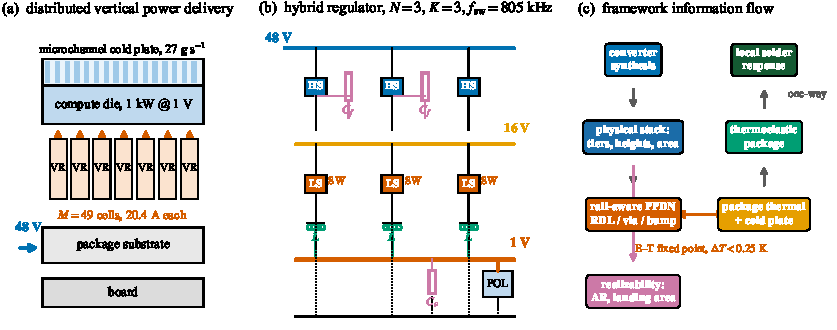
\includegraphics[width=\textwidth]{fig1_system.pdf}
\caption{(a) Distributed vertical power delivery: $M{=}49$ regulator cells convert 48\,V to
1\,V beneath or behind the compute die, so the high-current rail travels micrometres. (b) The
synthesised hybrid regulator, a three-to-one switched-capacitor stage feeding a two-phase
buck stage, with the rail carried by each branch annotated. (c) Information flow of the
framework: converter synthesis and the component library determine an explicit physical
stack, which is shared by the electrical, thermal, mechanical and realizability models. The
electrical and thermal models are iterated to a fixed point; the converged field is applied
one-way to the mechanical model.}
\label{fig:system}
\end{figure*}

A hybrid converter is adopted, consistent with the topologies used for high step-down ratios
in DVPD~\cite{DSCH,DPMIH44,SC_example}. The synthesised architecture, denoted
$N{=}3$, $K{=}3$, $K_{A}{=}2$, comprises a three-to-one switched-capacitor stage feeding a
\emph{two-phase} buck stage with $K{=}3$ parallel inductor branches, as shown in
Fig.~\ref{fig:system}(b). The switched-capacitor stage divides the 48\,V input to a 16\,V
intermediate rail, relieving both the voltage stress on the buck switches and the extreme
duty cycle a direct 48\,V-to-1\,V buck would require; the resulting duty cycle is
$D = N V_{\mathrm{out}}/V_{\mathrm{in}} = 0.0625$. The $N$ switched-capacitor branches share
$N-1$ flying capacitors, and each of the $K$ inductor branches carries an inductor and a
low-side switch whose drain forms the switch node.

The buck stage operates in \emph{two} switching phases, not $K$. In phase~A the
$\lceil N/2 \rceil$ branches of that group conduct and the $K_{A}{=}2$ inductors they feed
are connected to the intermediate rail, while the remaining $K_{B} = K - K_{A} = 1$ inductor
freewheels; in phase~B the complementary set conducts and the roles reverse, which is what
balances the flying capacitors over a cycle. $K$ is therefore the number of parallel
inductor branches and $K_{A}$ the number of those branches driven in phase~A; neither is a
count of switching phases. Branch currents follow
$I_{\mathrm{branch},i} = I_{\mathrm{cell}} B_{i} / N$ with $\sum_i B_i = N$, which for
$\mathbf{B} = [1,1,1]$ gives $6.803$\,A in every branch. The implementation contains no
time-domain model of the two states---no phase displacement, dead time or per-state
capacitor solve---so no claim of interleaving is made.

% BEGIN final-lineage:physarch
\subsection{Physical architectures}\label{sec:physarch}
\begin{figure*}[!t]
\centering
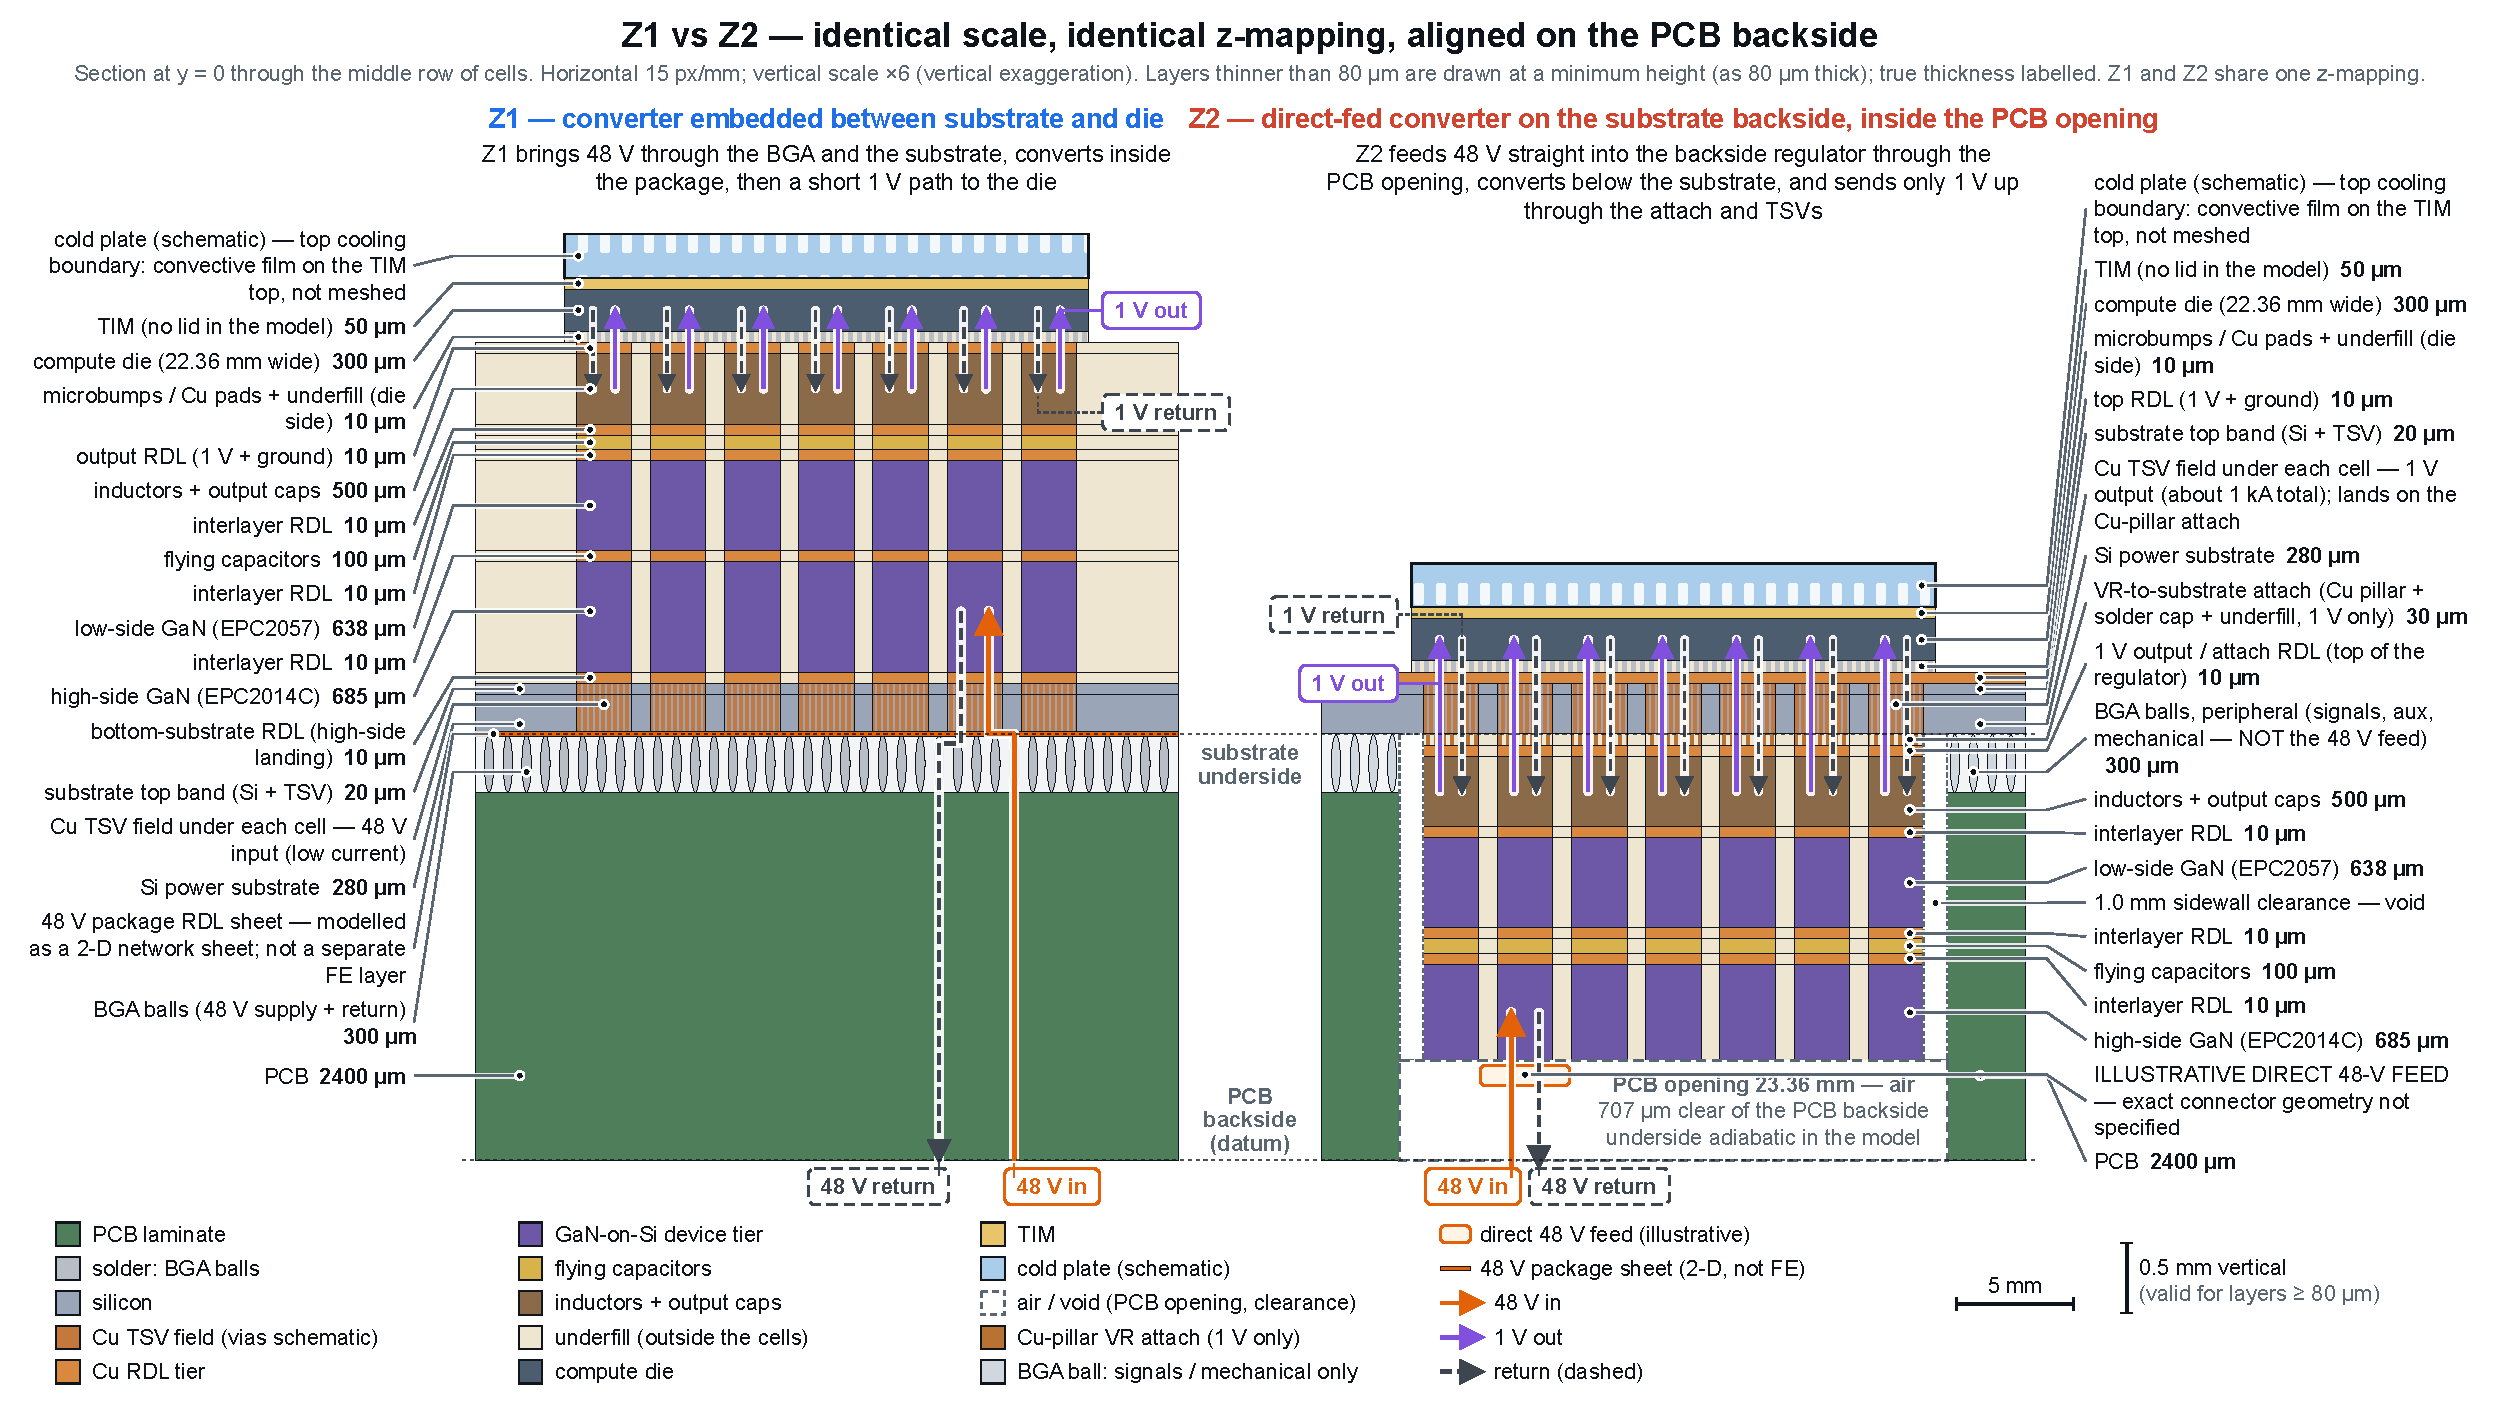
\includegraphics[width=\textwidth]{fig12_package_sections.pdf}
\caption{The two physical architectures at one scale, drawn from the solver mesh (layer heights
measured, not typed). Z1: the converter is embedded between substrate and die, and its 48\,V
arrives through the ball-grid array and the package 48\,V redistribution layer. Z2: the converter
hangs below a \SubZtwoUM\,$\mu$m substrate inside a \CutoutMM\,mm opening of the 2.4\,mm board,
with a \ClearanceMM\,mm void between the cell grid and the opening sidewall; its 48\,V enters
through an illustrative direct feed (the exact connector geometry is not specified), and only
1\,V crosses the substrate through the pillar attach and the TSV fields. The BGA balls of Z2
carry signals, auxiliary rails and mechanical support, not the 48\,V input.}
\label{fig:package}
\end{figure*}
\begin{figure*}[!t]
\centering
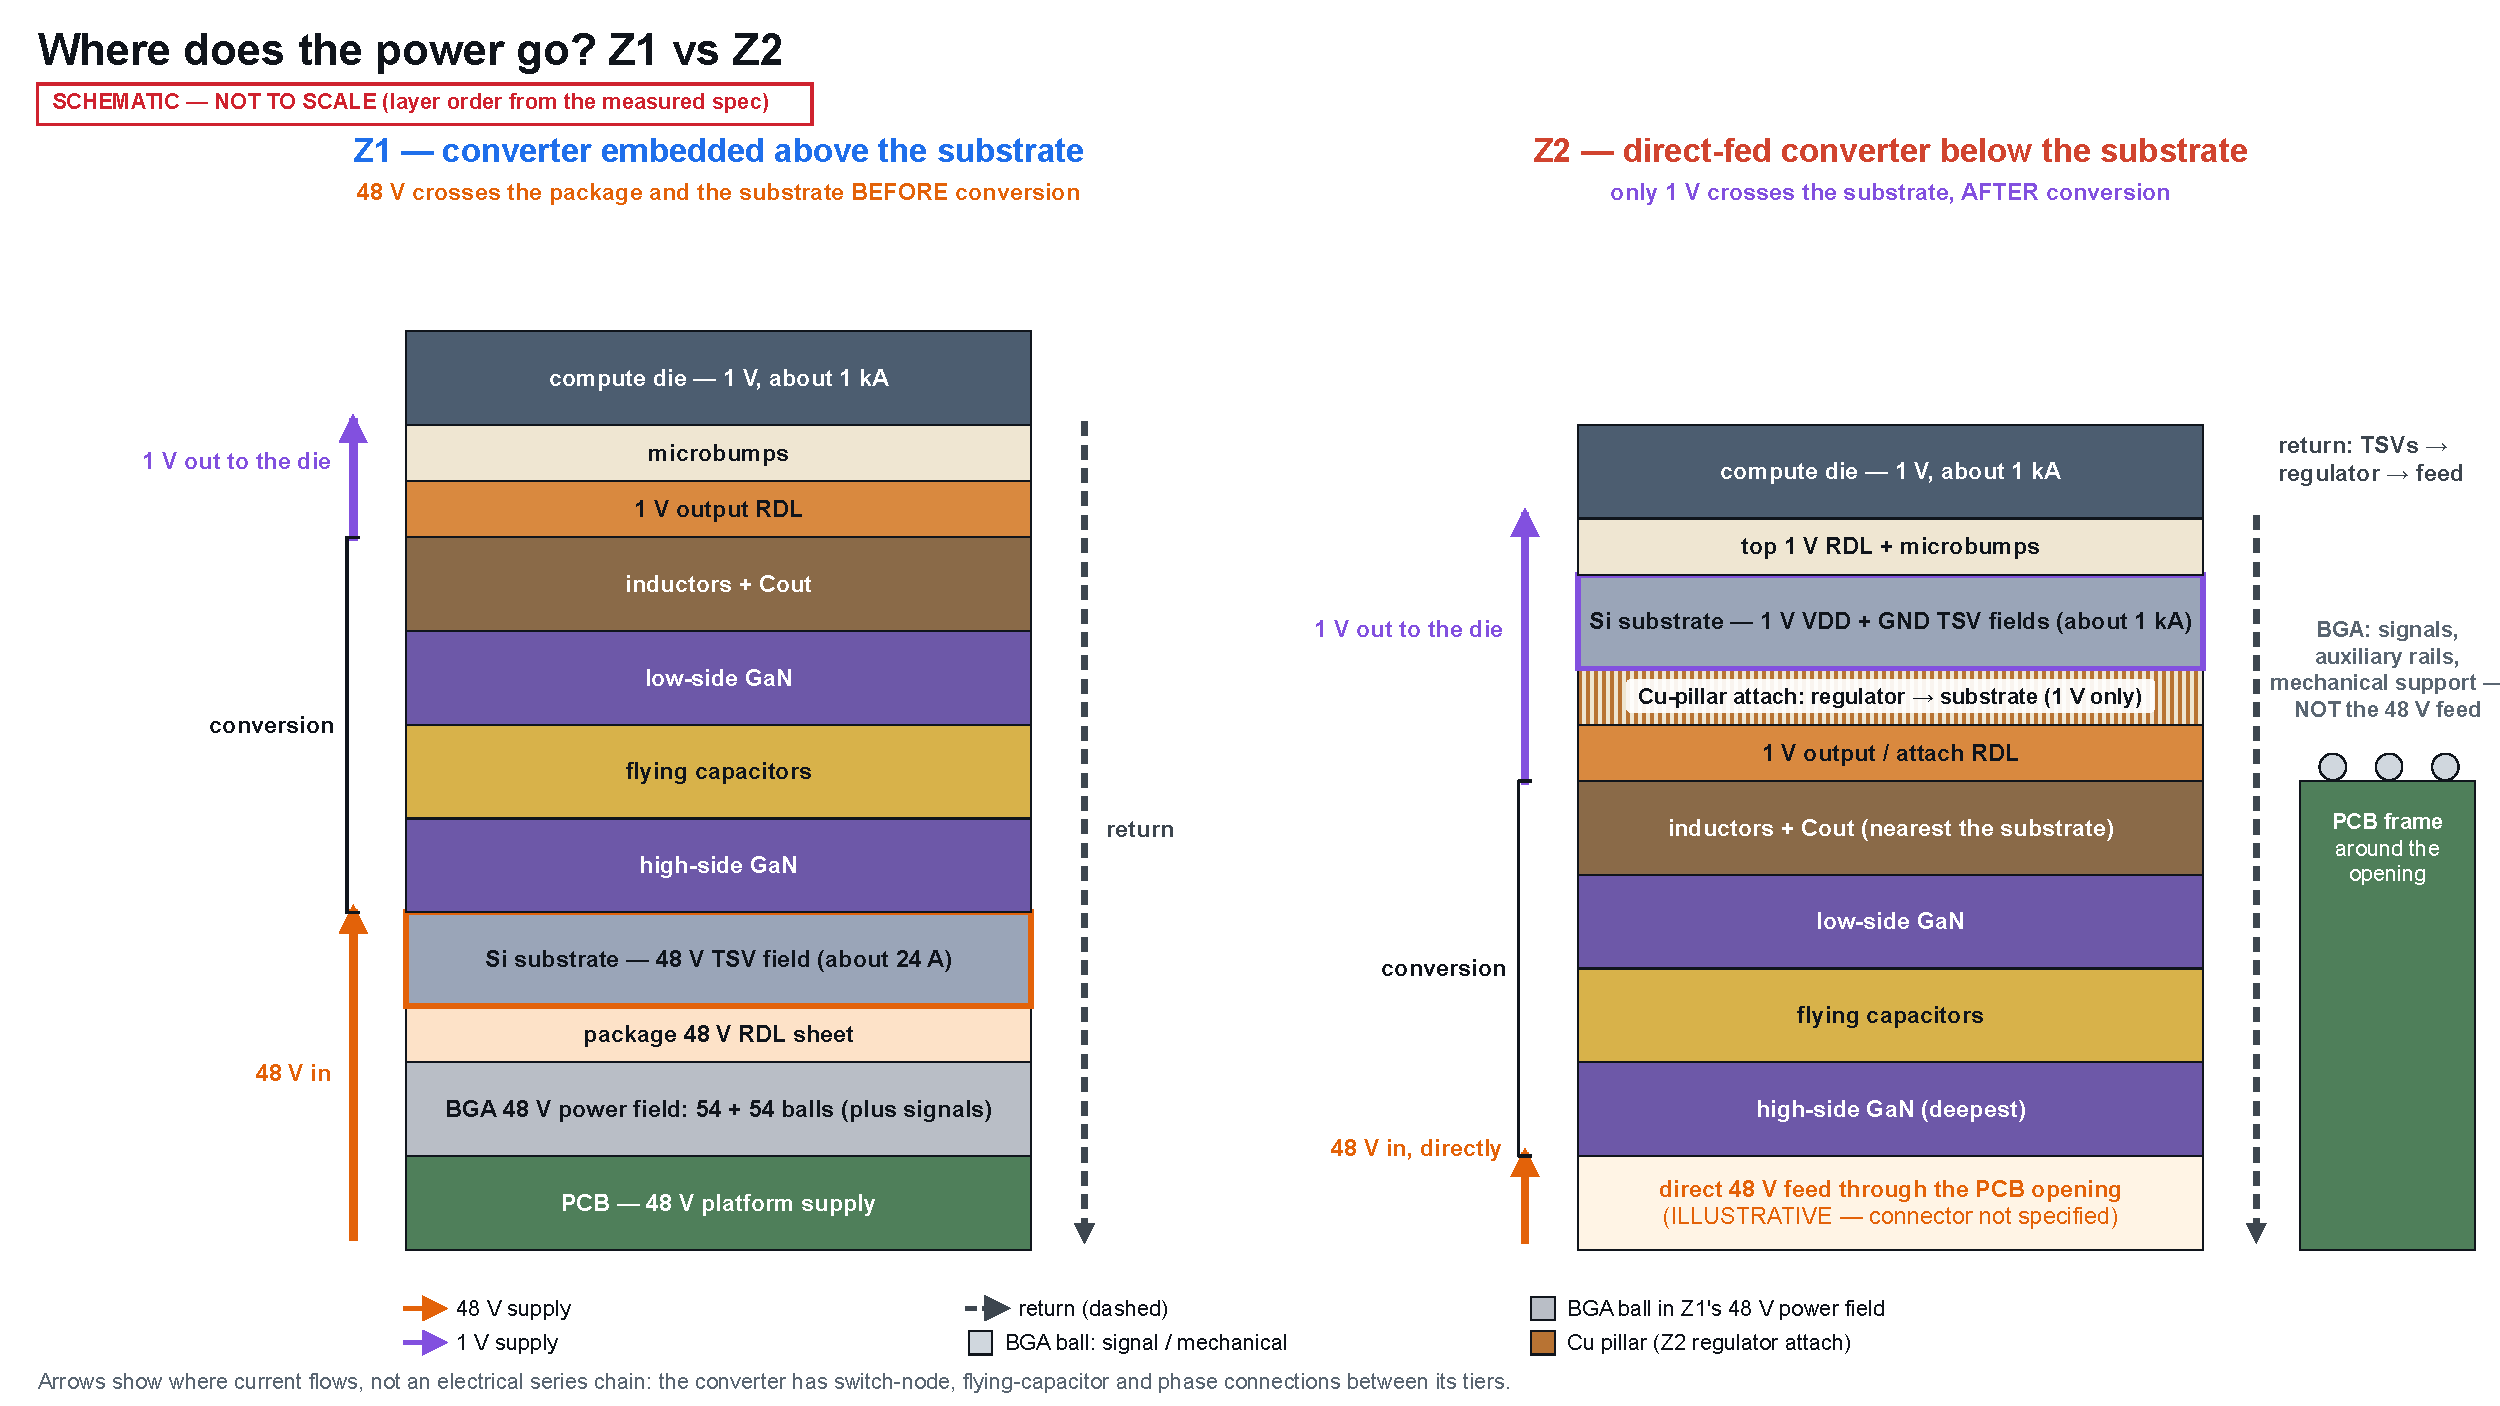
\includegraphics[width=\textwidth]{fig11_power_path.pdf}
\caption{Power paths, schematic (layer order from the measured specification, not to scale).
The Z2 stack is drawn in the order energy flows---direct input, high-side device, flying
capacitors, low-side stage, inductors and output capacitors, output and attach
redistribution, attach, substrate, top redistribution, die---which is not a series circuit:
switch-node, flying-capacitor, ground and phase connections run between non-adjacent tiers.}
\label{fig:powerpath}
\end{figure*}
Two physical integration alternatives are compared (Figs.~\ref{fig:package}
and~\ref{fig:powerpath}). Both were frozen in an architecture specification before any result in
this paper was computed, and their layer heights are measured on the solver mesh.

In the \emph{embedded} architecture (Z1), the platform 48\,V reaches the package through the
48\,V field of the ball-grid array (BGA), spreads in a package 48\,V redistribution layer (RDL)
and crosses the substrate through the through-silicon-via (TSV) field to the converter embedded
beneath the die; the 1\,V output then travels tens of micrometres through the output RDL and the
die-interface pads.

In the \emph{backside} architecture (Z2), the converter hangs below the substrate inside the
board opening. Its 48\,V input does not cross the package: it enters the regulator directly
through the opening by a dedicated external connection, and only the 1\,V output crosses the
substrate---through an explicit converter-to-substrate attach and the VDD and GND TSV fields---to
the top RDL and the die. This construction has a direct precedent~\cite{ArmCutoutVR2026}: a
vertical integrated regulator coupled to the side of the package substrate opposite the die,
located at least partly inside a circuit-board cutout, whose input power is provided by a
separate wire rather than through the board and substrate, and whose bumps to the substrate are
dedicated to the regulated output. That source is a construction precedent only: it states no
dimension, no performance figure and no qualification, and none is taken from it. A
die-backside regulator family~\cite{GoogleBacksideIVR2021} supplies the backside-RDL-to-TSV
output path as a close analog; it feeds its regulator through the package, so it is not a
precedent for the direct feed.

The BGA has two functions that an earlier representation of this study conflated. Its
\emph{mechanical field}---every package-to-board site that physically survives, \NsitesZone\
for Z1 and \NsitesZtwo\ for Z2 around the opening---carries signals, auxiliary rails, ground and
mechanical support, and the critical-joint search runs over all of it. Its \emph{48\,V power
field} is the subset that carries the regulator input: it exists in Z1 and is empty in Z2, a
property enforced by a regression test on the ledger.

The attach is a Cu pillar with a solder cap, \AttachH\,$\mu$m high (\AttachCu\,$\mu$m Cu and
\AttachCap\,$\mu$m cap), \AttachD\,$\mu$m in diameter at \AttachPitch\,$\mu$m pitch, in a VDD/GND
checkerboard under every cell footprint, with underfill: \AttachNbump\ pillars per rail per cell.
The geometry is that of a 30\,$\mu$m-pitch Cu-pillar microbump process on an organic
substrate~\cite{Au2016CuPillar30um}, a close analog; all-solder microbumps~\cite{Na2022SnMicrobump}
and heights of 20 and 40\,$\mu$m are carried as sensitivities (Table~\ref{tab:sources}). The
converter cells occupy $\pm$\FillExtentMM\,mm; the \ClearanceMM\,mm ring between them and the
opening sidewall is void, so the converter is not bonded to the board, and encapsulant fills only
the space between the cells. The previous construction filled the opening to its sidewall,
contradicting the stack specification; it is retained only as a sensitivity.

From the direct input upward, the Z2 stack runs high-side device, interlayer redistribution,
flying capacitors, interlayer redistribution, low-side stage, interlayer redistribution,
inductors and output capacitors, output and attach redistribution, attach, substrate with its
TSV fields, top redistribution, die interface and die. That sequence is the order in which
energy flows, not a series circuit: the switch-node, flying-capacitor, ground and phase
connections run between non-adjacent tiers inside the regulator, and the ledger assigns each
of them to its own conductor.

Finally, a control is kept to separate the effect of the opening and the ball placement from the
effect of the feed: \emph{a controlled experiment that forces both architectures to use an
identical package-level 48\,V feed}. In it, the backside converter takes its 48\,V through the
same matched BGA count and a package 48\,V RDL. It is an experiment, not a construction, and is
reported separately (Sec.~\ref{sec:control}).

\begin{table}[!t]
\caption{Source hierarchy of the architecture definition (DIRECT: describes this
construction; CLOSE\_ANALOG: bounds a value here; CONTEXT\_ONLY: no value taken). No
dimension is copied from a drawing.}
\label{tab:sources}
\centering
\footnotesize
\setlength{\tabcolsep}{2.5pt}
\begin{tabular}{@{}L{3.0cm}L{2.2cm}L{2.6cm}@{}}
\toprule
Statement & Source & Class \\
\midrule
Regulator on the substrate backside, in a board cutout, fed by a separate wire, bumps dedicated to the regulated output & \cite{ArmCutoutVR2026} & DIRECT (construction only; no dimension, no performance) \\
Backside RDL carrying regulated power into substrate TSVs & \cite{GoogleBacksideIVR2021} & CLOSE\_ANALOG (fed through the package) \\
Attach: 15\,$\mu$m Cu pillar, 30\,$\mu$m pitch, solder cap & \cite{Au2016CuPillar30um} & CLOSE\_ANALOG \\
Attach bound: 30\,$\mu$m Sn microbump, 80\,$\mu$m pitch, 40\,$\mu$m high & \cite{Na2022SnMicrobump} & CLOSE\_ANALOG (bound) \\
Fine-pitch bonding and material systems & \cite{Lee2017CuPillarNCF,Dai2018MicroBump30um,Xu2026CuPillarReview} & CONTEXT\_ONLY \\
External feed loop resistance & none & swept, not assumed \\
Embedded-microchannel DVPD cooling & \cite{Choi2024ITherm,Choi2025SelfConsistent} & CONTEXT\_ONLY \\
\bottomrule
\end{tabular}
\end{table}

\subsection{Historical frozen representation}\label{sec:histrep}
The comparison that motivated this work was carried out on a frozen, physically unclosed
representation of the two alternatives (Fig.~\ref{fig:stack}). Its results are kept in
Sec.~\ref{sec:arch} only to show what the physical closure changed; no current result uses it.
\begin{figure*}[!t]
\centering
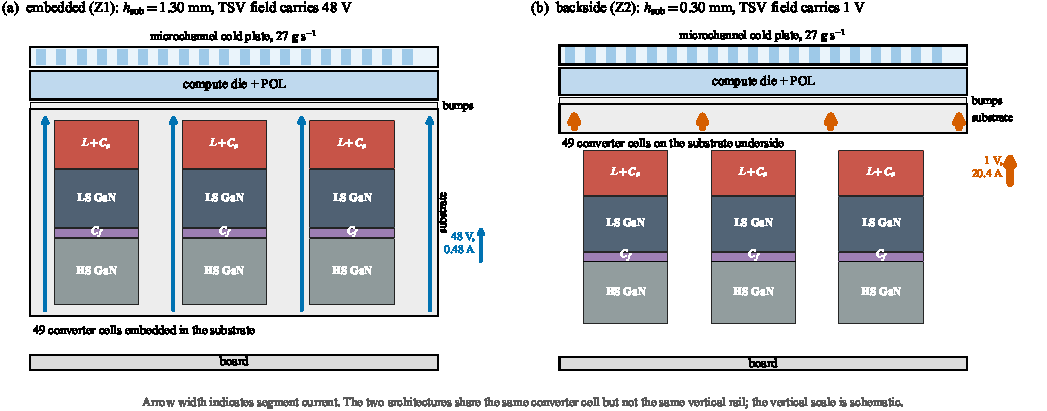
\includegraphics[width=0.94\textwidth]{fig2_stack.pdf}
\caption{Historical frozen representation, superseded by Figs.~\ref{fig:package} and~\ref{fig:powerpath}: stack and power path for the two integration alternatives. (a) Embedded:
the low-side devices, flying capacitors and inductors---$1226$\,\textmu m of the
$1921$\,\textmu m component stack at the frozen device heights, $1258$ of $1953$\,\textmu m
at the selected ones---are embedded in the $1.30$\,mm substrate, which they fill
together with the $74$\,\textmu m through-substrate field; that field carries the 48\,V input
rail. The $685$\,\textmu m high-side device is flip-chipped below the substrate and is outside
the modelled domain. (b) Backside: the converter medium occupies a continuous layer below a
$0.30$\,mm substrate and the field carries the 1\,V output rail at the full cell current; the
lateral subdivision of that layer into cells, and the board interface beneath it, are not
resolved. Arrow width indicates segment current on a logarithmic scale. The two are
electrically distinct despite sharing the same converter.}
\label{fig:stack}
\end{figure*}

The distinction between the two integration alternatives is electrical as well as geometric.
In the \emph{embedded} architecture (Z1) the low-side devices, flying capacitors and
inductors are embedded in the package substrate beneath the compute die. They occupy
$1226$\,\textmu m of the $1.30$\,mm substrate at the frozen device heights ($1258$ at the
selected ones, which the $1.30$\,mm substrate no longer accommodates) and the remaining
$74$\,\textmu m is the
through-substrate field, which carries the 48\,V input rail at low current; the substrate
budget therefore closes exactly. Following the reference
architecture~\cite{Krishnakumar2026DVPD}, the $685$\,\textmu m high-side device is
flip-chipped below the substrate; it lies outside the modelled domain, and its loss is
deposited in the embedded band. In the \emph{backside} architecture (Z2) the converter medium
lies below the substrate and is connected through the full $0.30$\,mm, so the identical field
carries the 1\,V output rail at the full cell current. That medium is represented as a
continuous layer rather than as 49 discrete cells, and the interface between it and the board
is not defined; both were limitations of that frozen geometry rather than properties of the
architecture, and the physical architectures above resolve them, and Sec.~\ref{sec:backside-limit} quantifies their effect. The vertical interconnect is therefore not common mode between the two and cannot be
treated as such. Both are shown in Fig.~\ref{fig:stack}.
% END final-lineage:physarch

A power-die variant and a 2.5-D lateral variant were also formulated. Neither is reported
here: no source available to this work establishes the power-die construction, and its
ranking depends on which construction is assumed.

\subsection{Coupled design variables}
The variables that couple the domains are the number of regulator cells, the substrate
thickness, the assignment of components to tiers, the vertical interconnect geometry and
pitch, and the cooling boundary. Each appears in more than one domain. The tier assignment,
for example, simultaneously sets the interconnect loss, the height budget, the depth at which
heat is deposited and the distribution of stiffness through the stack.

\section{Converter, Interconnect and Power-Delivery Models}\label{sec:elec}

\subsection{Regulator synthesis}
The converter is synthesised rather than assumed. Inputs are the per-cell output current
$I_{\mathrm{cell}}$, the input and output voltages, a target current density
$J_{\mathrm{t}} = 3.5$\,A\,mm$^{-2}$ that sets the area budget, and the component libraries.
The search enumerates hybrid architectures over the stage count $N$, the inductor-branch
count $K$, the phase-A branch count $K_{A}$ (restricted in the present implementation to
$\lceil K/2 \rceil$) and the branch-allocation vector $\mathbf{B}$, where $B_i$ is the number
of switched-capacitor branches feeding inductor $i$ and $\sum_i B_i = N$. For each
candidate it filters the device library by blocking voltage and current capability,
\begin{equation}
V_{\mathrm{DS,max}}^{\mathrm{HS}} \ge \frac{V_{\mathrm{in}}}{N}, \quad
V_{\mathrm{DS,max}}^{\mathrm{LS}} \ge V_{\mathrm{out}}, \quad
I_{\mathrm{D}}^{\mathrm{HS}} \ge \frac{I_{\mathrm{cell}}}{N},
\label{eq:filter}
\end{equation}
with the low-side devices filtered at $I_{\mathrm{D}} \ge I_{\mathrm{cell}}B_{\max}/N$. The
switching frequency is selected as the minimum satisfying the ripple constraint, since the
loss is monotonic in $f_{\mathrm{sw}}$ above that point. The candidate of lowest total loss
that satisfies both the area budget and the ripple constraint is retained. For the present
specification this returns $N3K3K_{A}2$ at $f_{\mathrm{sw}} = 805.17$\,kHz from a 90-device
library, using the devices and passives listed in Table~\ref{tab:spec}.

\subsection{Converter loss model}
The losses evaluated are exactly those the synthesis model implements; no mechanism is added
on the grounds of being conventional. The \emph{summed output} current ripple---$K_{A}$
inductors driven from the intermediate rail while $K-K_{A}$ freewheel---with
$k_{\mathrm{c}}$ the inter-inductor coupling coefficient, is
\begin{equation}
\Delta i_{\phi} = \frac{1}{1+k_{\mathrm{c}}(K-1)}\,
\frac{D}{f_{\mathrm{sw}} L}\left(\frac{V_{\mathrm{in}}}{N}K_{A} - V_{\mathrm{out}}K\right),
\label{eq:ripple}
\end{equation}
where the $K_{A}V_{\mathrm{in}}/N$ term is the contribution of the branches connected to the
intermediate rail in that state and the $KV_{\mathrm{out}}$ term is the output voltage
sustained by all $K$ inductors in every state. This gives the r.m.s. cell current
$I_{\mathrm{rms}} = \sqrt{I_{\mathrm{cell}}^{2} + \Delta i_{\phi}^{2}/12}$ and the output
voltage ripple $\Delta V_{\mathrm{out}} = |\Delta i_{\phi}|/(8 f_{\mathrm{sw}} C_{\mathrm{o}})$.

Conduction loss is evaluated in closed form over the hybrid network. With
$\mathcal{B} = \sum_{i} B_{i}^{2}$, $B_{k}$ the final conversion ratio and
$\kappa = (V_{\mathrm{out}}/V_{\mathrm{in}})I_{\mathrm{rms}}^{2}$,
\begin{equation}
\begin{aligned}
P_{\mathrm{cond}} = \kappa \Bigg[ &R_{\mathrm{on}}^{\mathrm{HS}}
 + 2\!\left(1-\tfrac{1}{N}\right)\!R_{\mathrm{ESR}} \\
 &+ \left(\frac{V_{\mathrm{in}}}{N^{2}V_{\mathrm{out}}}
   \big(R_{\mathrm{DCR}} + R_{\mathrm{on}}^{\mathrm{LS}}\big)
   + \frac{2R_{\mathrm{on}}^{\mathrm{LS}}}{N}\right)\!\mathcal{B}
 - \Gamma \Bigg],
\end{aligned}
\label{eq:pcond}
\end{equation}
where $\Gamma = (4B_{k}-1)R_{\mathrm{on}}^{\mathrm{LS}}/N$ for $B_{k}>1$ and
$3R_{\mathrm{on}}^{\mathrm{LS}}/N$ otherwise. The four bracketed groups are attributed
respectively to the high-side switches, the flying capacitors, the inductor winding
resistance and the low-side switches, which is how the loss ledger of
Section~\ref{sec:arch} is decomposed; the decomposition is checked against the aggregate of
\eqref{eq:pcond} to machine precision on every evaluation and the run is rejected if it does
not reproduce it.

Switching loss comprises three terms, evaluated by the plateau-voltage
method~\cite{efficiency}. With the gate-drive current
$I_{\mathrm{g}} = (V_{\mathrm{gs}} - \tfrac{1}{2}(V_{\mathrm{th}}+V_{\mathrm{pl}}))/
(R_{\mathrm{g}}+R_{\mathrm{drv}})$,
\begin{align}
P_{\mathrm{sw}} &= f_{\mathrm{sw}}\!\left(\frac{V_{\mathrm{in}}}{N}-V_{\mathrm{out}}\right)
 I_{\mathrm{rms}}\,\frac{Q_{\mathrm{GD}}+Q_{\mathrm{G}}}{I_{\mathrm{g}}},
\label{eq:psw}\\
P_{\mathrm{gate}} &= f_{\mathrm{sw}}\!\left(N C_{\mathrm{G}}^{\mathrm{HS}}
 + K C_{\mathrm{G}}^{\mathrm{LS}}\right) V_{\mathrm{gs}}^{2},
\label{eq:pgate}\\
P_{\mathrm{C_{oss}}} &= \frac{f_{\mathrm{sw}}}{2}\!\left[
 N C_{\mathrm{oss}}^{\mathrm{HS}}\!\left(\frac{V_{\mathrm{in}}}{N}-V_{\mathrm{out}}\right)^{2}
 \!\!+ K C_{\mathrm{oss}}^{\mathrm{LS}} V_{\mathrm{out}}^{2}\right]\!.
\label{eq:pcoss}
\end{align}

Two omissions are deliberate and are stated rather than left implicit. Inductor core loss is
not evaluated: the component library carries Steinmetz coefficients, but the synthesis model
consumes only the winding resistance $R_{\mathrm{DCR}}$, so only conduction loss in the
inductor is reported. Capacitor loss is likewise represented by the equivalent series
resistance alone. Both omissions bias the reported dissipation downward and act on the same
component set in both architectures. They are therefore not expected to alter the reported
ordering, although the two architectures do not operate at the same temperature, so exact
cancellation is not asserted. The absolute efficiency remains underestimated.

Temperature dependence enters through two coefficients. The switch on-resistance and the
inductor winding resistance are scaled from their datasheet reference of $25\,^{\circ}$C, and
the copper resistivity of every interconnect from $20\,^{\circ}$C,
\begin{equation}
\begin{aligned}
R_{\mathrm{on}}(T) &= R_{\mathrm{on}}^{25}\!\left[1+\alpha_{\mathrm{GaN}}(T-25)\right],\\
\rho(T) &= \rho_{20}\!\left[1+\alpha_{\mathrm{Cu}}(T-20)\right],
\end{aligned}
\label{eq:tdep}
\end{equation}
with $\alpha_{\mathrm{Cu}} = 3.93\times10^{-3}$\,K$^{-1}$ and
$\alpha_{\mathrm{GaN}} = 7.5\times10^{-3}$\,K$^{-1}$. The second is an \emph{adopted
calibration coefficient, not a sourced material constant}: the device tables used
here~\cite{EPC2014C,EPC2057} carry no temperature columns, so no coefficient for the two
selected parts can be cited. The value reproduces the normalised on-resistance rise published
for enhancement-mode GaN parts, about $1.75\times$ at $125\,^{\circ}$C, and is treated
throughout as a sensitivity parameter. It is the input to which the electrical result is most
sensitive: on the frozen pair a $\pm20$\,\% change moves converter loss by $\mp5.8$\,\%, and
a $\pm33$\,\% change swept through the converged electrical--thermal loop moves peak
temperature by at most $1.2$\,K. The Z1/Z2 loss ordering is preserved at every value tested,
so no ordering reported here depends on it; absolute efficiency inferred from this work
inherits its uncertainty.

\subsection{Rail-aware current assignment}
\begin{figure*}[!t]
\centering
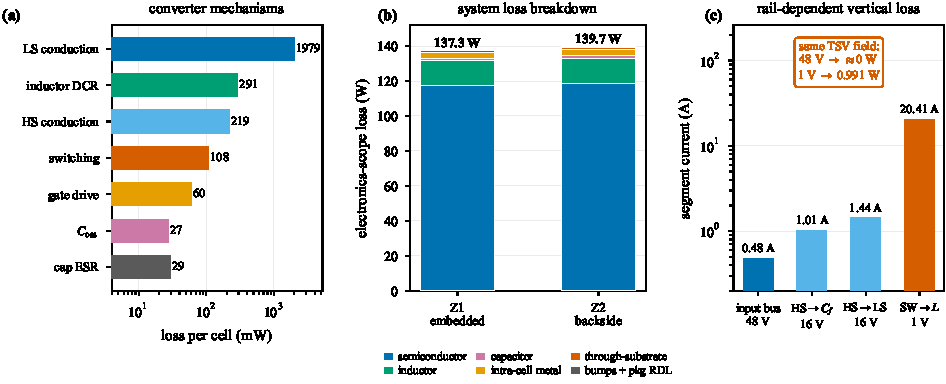
\includegraphics[width=\textwidth]{fig3_loss.pdf}
\caption{(a) Converter loss mechanisms evaluated by \eqref{eq:pcond}--\eqref{eq:pcoss} for
one cell, showing the dominance of low-side conduction at a duty cycle of $0.0625$. (b)
Electronics-scope loss breakdown for the frozen pair, separating converter losses from package
losses. (c) Segment current and the resulting vertical interconnect loss: the same
through-substrate field dissipates essentially nothing carrying 48\,V and $0.991$\,W carrying
1\,V, which is why the interconnect is not common mode across architectures.}
\label{fig:loss}
\end{figure*}

The converter is represented as a terminal graph whose edges are the physical connections
between component terminals. Each edge is assigned the rail it carries and the current that
rail carries, rather than a representative cell current. For the synthesised topology the
input bus carries $I_{\mathrm{in}} = P_{\mathrm{in}}/V_{\mathrm{in}} = 0.478$\,A, the
high-side to flying-capacitor edge $1.015$\,A, the mid-rail edge $1.435$\,A, and the switch
node and output edges the full $20.408$\,A. The segment currents within one cell therefore
span nearly two orders of magnitude, as shown in Fig.~\ref{fig:loss}(c). Because segment loss
scales as the square of the current, assigning one representative current to all vertical
segments misstates the vertical loss by a correspondingly large and partition-dependent
factor.

The switch-node edge is an aggregate over the $K$ phases. Per device it carries
$I_{\mathrm{cell}}/K = 6.803$\,A, within the $9.6$\,A continuous rating of the selected
low-side part, and there are $K$ such devices each presenting its own drain land.

\subsection{Vertical and lateral interconnect}
Each vertical field is provisioned from the current it carries and the design current
density $J_{\mathrm{d}} = 1\times10^{8}$\,A\,m$^{-2}$. For a via of radius $r$ with liner
thickness $t_{\ell}$ the conducting area is
$A_{\mathrm{cu}} = \pi(r-t_{\ell})^{2}$ and
\begin{equation}
n_{\mathrm{req}} = \left\lceil \frac{I}{J_{\mathrm{d}} A_{\mathrm{cu}}} \right\rceil, \qquad
n_{\mathrm{req}} \le n_{\mathrm{alloc}} \le n_{\mathrm{avail}},
\label{eq:nreq}
\end{equation}
where $n_{\mathrm{alloc}}$ is the count the allocation policy instantiates and
$n_{\mathrm{avail}} = \lfloor \eta A_{\mathrm{land}}/p^{2}\rfloor$ is the count the available
landing area $A_{\mathrm{land}}$ admits at pitch $p$ with areal packing efficiency $\eta$.
The field resistance uses the allocated count,
\begin{equation}
R_{\mathrm{field}} = \frac{R_{\mathrm{single}}}{n_{\mathrm{alloc}}}
 = \frac{\rho(T)\,h}{A_{\mathrm{cu}}\, n_{\mathrm{alloc}}},
\label{eq:rfield}
\end{equation}
for a via of height $h$. Using $n_{\mathrm{req}}$ in \eqref{eq:rfield} instead states an
allocation policy as though it were a physical law.

Two consequences are used later. Under minimum-capability provisioning, for which
$n_{\mathrm{alloc}} = n_{\mathrm{req}}$, the copper fraction of the field is
\begin{equation}
\varphi_{\mathrm{cu}} = \frac{n_{\mathrm{req}} A_{\mathrm{cu}}}{A_{\mathrm{field}}}
 \simeq \frac{I}{J_{\mathrm{d}} A_{\mathrm{field}}},
\label{eq:phi}
\end{equation}
which is independent of $r$: enlarging a via changes the required count and leaves the field
resistance, the homogenised conductivity and the effective stiffness essentially unchanged.
And the legal pitch follows from the additive spacing rule
$p = \max(2r + s_{\min},\, 2r(1+\kappa_{\mathrm{koz}}))$ with $s_{\min} = 30$\,\textmu m, so
the ratio $n_{\mathrm{req}}/n_{\mathrm{avail}}$ \emph{improves} as $r$ increases, which is
the opposite of the intuition that finer vias relieve a congested field.

\begin{table}[!t]
\caption{Comparison on the frozen repartitioned pair. \textbf{Every value in this
table is a frozen Phase-0M-R3C result and is retained as the historical baseline
against which the physical hardening is measured; none of it is a current physical
result.} The interconnect rows in particular predate the corrected package model:
the package redistribution network was subsequently rebuilt with voltage-fed BGA
branches, a separately solved return conductor and finite contacts, which showed
that equal ball-current sharing --- assumed when these rows were produced --- does
not hold. The superseded rows are \emph{Intra-cell metal}, \emph{Vertical
transitions} and \emph{Bumps + package RDL}; the corresponding terms are presently
carried as \textsc{open} in the physical loss ledger rather than replaced by new
numbers, because their currents are defined only per named scenario. The
corner-joint displacement driver $\du$ and the local inelastic response
$\Delta\varepsilon_{\mathrm{in}}$ are separate quantities and are reported
separately: $\du$ is the in-plane displacement the global solve imposes on the
joint, $\Delta\varepsilon_{\mathrm{in}}$ the dimensionless per-cycle strain
increment the viscoplastic submodel returns for it. Both architectures are
geometrically realizable and process-conditional; neither is qualified.}
\label{tab:final}
\centering
\footnotesize
\begin{tabular}{@{}lrr@{}}
\toprule
Quantity & Z1 embedded & Z2 backside \\
\midrule
\multicolumn{3}{@{}l}{\emph{Electronics-scope loss}}\\
Low-side conduction (W) & $96.956$ & $98.074$ \\
High-side conduction (W) & $10.736$ & $10.859$ \\
Inductor winding (W) & $14.266$ & $14.370$ \\
Capacitor ESR (W) & $1.440$ & $1.440$ \\
Switching, gate, $C_{\mathrm{oss}}$ (W) & $9.602$ & $9.602$ \\
Intra-cell metal (W) & $3.601$ & $3.627$ \\
Vertical transitions (W) & $0.011$ & $0.011$ \\
Through-substrate field (W) & $\sim0$ & $\mathbf{0.991}$ \\
Bumps + package RDL (W) & $0.680$ & $0.685$ \\
\textbf{Total} & $\mathbf{137.292}$ & $\mathbf{139.659}$ \\
Pump power, facility scope (W) & $14.696$ & $14.696$ \\
\midrule
\multicolumn{3}{@{}l}{\emph{Thermal and mechanical}}\\
Peak temperature ($^{\circ}$C) & $118.32$ & $\mathbf{126.46}$ \\
Mean die temperature ($^{\circ}$C) & $93.41$ & $95.41$ \\
Die warpage, peak-to-valley (\textmu m) & $41.616$ & $38.916$ \\
Package warpage, P--V (\textmu m) & $77.024$ & $72.039$ \\
Corner-joint temperature $T_{\mathrm{j}}$ ($^{\circ}$C) & $112.75$ & $\mathbf{120.30}$ \\
E--T iterations / energy residual & $3$ / $0$\,\% & $3$ / $0$\,\% \\
\midrule
\multicolumn{3}{@{}l}{\emph{Local joint}}\\
Displacement driver $\du$ (\textmu m) & $4.6252$ & $\mathbf{3.8714}$ \\
Inelastic response $\Delta\varepsilon_{\mathrm{in}}$ ($\times10^{-2}$/cycle)
 & $1.4072$ & $\mathbf{1.1478}$ \\
Inelastic strain range ($\times10^{-3}$) & $6.898$ & $5.628$ \\
Inelastic work (MJ\,m$^{-3}$) & $1.0853$ & $0.9309$ \\
Cycle-to-cycle change, last pair & $0.04$\,\% & $0.06$\,\% \\
\midrule
Driver ratio $D_{u}$ & \multicolumn{2}{c}{$1.1947$} \\
Response ratio $D_{\varepsilon}$ & \multicolumn{2}{c}{$\mathbf{1.2260}$} \\
Worst via aspect ratio & \multicolumn{2}{c}{$0.833$} \\
Worst provisioning ratio & \multicolumn{2}{c}{$0.633$} \\
\bottomrule
\end{tabular}
\end{table}

Lateral distribution is treated as a sheet problem. For a segment of length $\ell$ carrying
current $I$ across $n_{L}$ metal layers of thickness $t_{\mathrm{cu}}$,
\begin{equation}
w_{\mathrm{req}} = \frac{I}{J_{\mathrm{d}} t_{\mathrm{cu}} n_{L}}, \qquad
R = \frac{\rho(T)\,\ell}{n_{L} w t_{\mathrm{cu}}}, \qquad w \le w_{\mathrm{avail}},
\label{eq:rdl}
\end{equation}
and a segment for which $w_{\mathrm{req}} > w_{\mathrm{avail}}$ is infeasible rather than
merely lossy. Every segment contributes $P = I_{\mathrm{rms}}^{2}R$ to the loss ledger and,
through its position in the stack, to the volumetric heat source of
Section~\ref{sec:thermech}. Supply and return are both represented: the ledger separates
intra-cell metal, the vertical transitions, the through-substrate field, the bump field and
the package redistribution network, and Table~\ref{tab:final} reports them separately.

\subsection{Conductor-plane topology and realizability}
\begin{figure*}[!t]
\centering
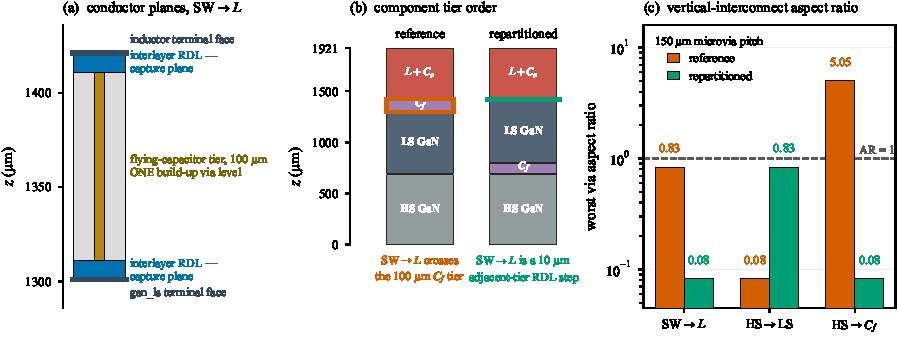
\includegraphics[width=\textwidth]{fig4_realizability.pdf}
\caption{Physical realizability of the vertical interconnect. (a) Conductor-plane sequence
for the switch-node connection: three material layers separate the terminal faces, but the
interlayer redistribution layers are capture planes, so one build-up via level is required.
(b) Component tier order before and after the repartition; exchanging the low-side switches
with the flying capacitors leaves the component set, per-tier areas and stack height
unchanged. (c) Worst via aspect ratio per vertical net at a source-bounded microvia pitch:
the $606$\,\textmu m crossing required by the reference order is eliminated and the worst
aspect ratio falls from $5.05$ to $0.833$ at the frozen device heights. The reference
order's worst net crosses the low-side tier, so with the selected EPC2057 height
($638$\,\textmu m) the figure becomes $5.32$ to $0.833$; the repartitioned value is
unchanged because it crosses the capacitor tier.}
\label{fig:realize}
\end{figure*}

Whether a connection between two components in different tiers requires one via level or
several is determined by the \emph{conductor-plane} sequence of the stack, not by the number
of material layers between them. An interlayer redistribution layer is patterned copper and
serves as a capture plane on which a microvia lands; only a region containing no conductor
plane requires a via to cross it. For the switch-node connection in the reference tier order
the sequence is: device terminal face, interlayer redistribution layer, flying-capacitor
power layer, interlayer redistribution layer, device terminal face. Three material layers
separate the two terminal faces, but only one---the component tier---is a dielectric region
without an internal conductor plane. One build-up via level is therefore required, of depth
equal to that tier, as shown in Fig.~\ref{fig:realize}(a).

Feasibility is then evaluated per segment against four conditions: the count condition
\eqref{eq:nreq}; the pitch rule; the aspect ratio $\mathrm{AR} = h_{\mathrm{diel}}/d$ of each
via level against what the build-up process admits; and the landing area, which is a
property of the connected device rather than of the cell. The low-side transistor used here
is supplied as a bare die with four solder bars on a $1.5 \times 1.2$\,mm
footprint~\cite{EPC2057}, so its switch node is presented on at most a quarter of the die
area.

Throughout, the provisioning state of \eqref{eq:nreq} and the manufacturing state are
reported separately. $n_{\mathrm{req}}$ is a conservative design-side allocation evaluated at
$J_{\mathrm{d}}$; no current allowable has been sourced for the build-up microvia technology
considered, so $n_{\mathrm{req}}$ is never presented as a statement of what manufacturing
requires.
% BEGIN final-lineage:pdn
\subsection{Package power-delivery network closure}\label{sec:pdnclosure}
Only Z1 carries its 48\,V input through the package. Its 48\,V package redistribution network is
solved as two separate resistive sheets, supply and return, each fed from a rail node through
the individual series resistance of every ball-grid-array ball and a finite-area contact. Ball
currents are therefore an output of the solution rather than an imposed equal share, and under a
uniform cell load they are markedly unequal, so a count sized from the total current divided by
the ball count understates the most heavily loaded ball. Each regulator cell draws its input
through the 0.2\,mm input pad of the converter layout, not through the whole cell footprint. The
sheet is discretised by cell-centred finite volumes on a tensor grid whose faces coincide with
every pad edge and are graded toward every ball edge; on a uniform grid the pad boundaries fall
between nodes, the resulting error is first order, and the embedded network failed to converge,
whereas on the aligned grid every network converges to within 1\,\% on effective resistance,
dissipation, maximum cell drop, peak ball current and peak-to-mean ball current between the two
finest levels. The ball count is selected by enumerating every legal mirror-symmetric even count,
solving the network at each, and verifying the candidate minimum on the resolved grid; the peak
ball current is not monotone in the count, because the selected sites change with it. A matched
count of \NballMatched\ balls per rail satisfies the 1.5\,A-per-ball provisioning criterion in
the continuous-input scenario; that criterion is an engineering provisioning rule, not a
reliability allowable. The resulting loop resistance is \RloopZone\,m$\Omega$ for Z1; the same
network on the opening geometry, which only the BGA-fed control uses, gives
\RloopZtwo\,m$\Omega$. The direct-fed Z2 has no package 48\,V network, and its ledger carries no
package 48\,V ball or RDL term. The frozen electrical ledger at the converged electrothermal state
is given in Table~\ref{tab:ledger}.
% GENERATED by scripts/final_closure_manuscript_tables.py
\begin{table}[!t]
\caption{Frozen physical electrical ledger at the converged E--T state, HV-S0, inside the package-internal boundary (Z2 from the regulator's 48\,V input terminals, Z1 from the BGA pads). Every conductor has exactly one owner; --: structurally absent (no package 48\,V path in the direct-fed Z2, no attach tier in Z1). The control is the BGA-fed Z2 of Sec.~\ref{sec:control}. The direct-fed Z2's external feed adds $I_{48,\mathrm{rms}}^{2}R$ outside this boundary, 0.572\,W per m$\Omega$ of loop resistance here (Sec.~\ref{sec:directfeed}).}
\label{tab:ledger}
\centering
\footnotesize
\setlength{\tabcolsep}{3pt}
\begin{tabular}{@{}L{4.1cm}rrr@{}}
\toprule
Term (W) & Z1 & Z2 & control \\
\midrule
High-side GaN (cond.+sw.+gate+$C_{\mathrm{oss}}$) & 21.404 & 21.438 & 21.447 \\
Low-side GaN conduction & 105.732 & 105.418 & 105.493 \\
Inductor DCR & 14.376 & 14.635 & 14.641 \\
Capacitor ESR & 1.440 & 1.440 & 1.440 \\
Intra-VR metal (R0 traces + R2 plane) & 1.895 & 1.910 & 1.911 \\
Intra-VR via stacks & 2.346 & 2.364 & 2.365 \\
Package 48\,V RDL, supply + return & 1.802 & -- & 1.159 \\
48\,V BGA balls, supply + return & 0.017 & -- & 0.011 \\
VR-to-substrate attach, VDD + GND & -- & 0.234 & 0.234 \\
TSV field (Z1: 48\,V; Z2: 1\,V), VDD + GND & 0.000 & 0.555 & 0.555 \\
Source Cu pads, VDD + GND & 0.044 & 0.044 & 0.044 \\
\midrule
Total (package-internal) & 149.057 & 148.038 & 149.301 \\
\bottomrule
\end{tabular}
\end{table}


\subsection{Direct-feed boundary and requirement}\label{sec:directfeed}
Two boundaries are used. The \emph{package-internal} ledger of Z2 starts at the regulator's 48\,V
input terminals and contains the converter losses, the regulator's internal redistribution and
vias, the output plane, the attach, the TSV fields, the top RDL and the die-interface pads; that
of Z1 starts at its BGA pads on the board and contains the 48\,V balls, the package 48\,V RDL and
the 48\,V TSVs. The \emph{platform-inclusive} comparison adds the complete external 48\,V supply
and return loop of Z2, $R_{\mathrm{Z2,feed}}$, between the board-level 48\,V node common to both
architectures---where the board distribution of Z1 meets its balls---and the regulator's 49 input
terminals. Board distribution upstream of that node is common to both and excluded from both. No
source gives this loop resistance: the construction precedent names connector types only. No
value is therefore assumed; $R_{\mathrm{Z2,feed}}$ is swept from \FeedSweepLo\ to
\FeedSweepHi\,m$\Omega$ (\FeedSweepN\ log-spaced points), and the total Z2 loss
\begin{equation}
P_{\mathrm{Z2}}(R) = P_{\mathrm{int}}(I) + (k I)^{2} R,\qquad
48\,\mathrm{V}\cdot I = P_{\mathrm{load}} + P_{\mathrm{Z2}}(R),
\label{eq:feed}
\end{equation}
is solved for the self-consistent input current $I$ at the converged temperatures, with $k$ the
RMS-to-average ratio of the named scenario. For a fixed $P_{\mathrm{int}}$ the balance is a
quadratic in $I$ whose lower root is the operating point; $P_{\mathrm{int}}$ is re-evaluated at
that current until the balance closes, and above
$48^{2}/(4k^{2}(P_{\mathrm{load}}+P_{\mathrm{int}}))$ no operating point exists.
The crossover $R^{*}$ at which $P_{\mathrm{Z2}} = P_{\mathrm{Z1}}$ is found by bisection. It is
reported as a requirement on the feed, not as a property of any connector. The nominal analysis
deposits the feed loss outside the package; depositing it in the deepest converter tier is a
class-B variant (Sec.~\ref{sec:classb}).
% END final-lineage:pdn
\section{Thermal and Mechanical Formulation}\label{sec:thermech}

\subsection{Package thermal model}
Steady conduction is solved on the resolved package stack,
\begin{equation}
\nabla \cdot \left( \mathbf{k}\, \nabla T \right) + q'''\!\left(\mathbf{x}\right) = 0,
\label{eq:cond}
\end{equation}
with $\mathbf{k} = \mathrm{diag}(k_{x},k_{y},k_{z})$ an orthotropic conductivity tensor and
$q'''$ the volumetric source. Every loss term of Section~\ref{sec:elec} is deposited at the
layer in which it is generated: the converter losses in the converter band, the intra-cell
metal and vertical-transition losses in the tiers that carry them, the through-substrate
field loss in the via field, and the bump and package redistribution losses in their own
layers. The deposited total is checked against the electrical total on every solve to within
$10^{-6}$ relative, and a mismatch stops the run.

\begin{table}[!t]
\caption{Material properties of the package stack. Homogenised layers carry effective
properties derived from an explicitly meshed representative volume element.}
\label{tab:mat}
\centering
\footnotesize
\setlength{\tabcolsep}{3.5pt}
\begin{tabular}{@{}lcccc@{}}
\toprule
Layer / material & $E$ (GPa) & $\nu$ & $\alpha$ (ppm/K) & $k$ (W/m\,K) \\
\midrule
Silicon (cubic) & $C_{11}{=}166$ & $C_{12}{=}64$ & $2.6$ & $130$ \\
Copper & $110$ & $0.34$ & $16.66$ & $400$ \\
Through-substrate via field & \multicolumn{4}{c}{homogenised, $f_{\mathrm{Cu}}{=}0.196$} \\
Converter band (effective) & $120$ & $0.28$ & $6.0$ & $60$ \\
Interface / underfill & $8.0$ & $0.32$ & $30$ & $0.7$ \\
Thermal interface & $0.2$ & $0.45$ & $200$ & $3.0$ \\
Ball-grid-array field & $3.93$ & $0.35$ & $20.5$ & $9.82$ \\
Printed circuit board & $20$ & $0.20$ & $17$ & $0.3$ \\
\bottomrule
\end{tabular}
\end{table}

Layers containing regular arrays are homogenised rather than resolved. For a square-pitch
copper via array in silicon of area fraction $f = \pi d^{2}/(4p^{2})$, the through-thickness
conductivity follows the parallel rule $k_{z} = f k_{\mathrm{Cu}} + (1-f) k_{\mathrm{Si}}$,
exact for aligned continuous phases, and the effective expansion coefficient follows the
stiffness-weighted rule
$\alpha_{\mathrm{eff}} = (f E_{\mathrm{Cu}}\alpha_{\mathrm{Cu}} +
(1-f)E_{\mathrm{Si}}\alpha_{\mathrm{Si}})/(f E_{\mathrm{Cu}} + (1-f)E_{\mathrm{Si}})$. The
in-plane conductivity is taken from an explicitly meshed representative volume element
rather than from a closed form: for the bump fields the Maxwell--Garnett estimate agrees to
within $1.5$\,\%, but for the via arrays it is $11$ to $39$\,\% high, so the element result is
adopted. The interlayer redistribution layer, through which all dissipated power passes, is
strongly anisotropic, and treating it as isotropic shifts absolute temperatures by several
kelvin. Material properties are listed in Table~\ref{tab:mat}.

The unheated faces are treated as adiabatic on the sides, with natural convection of
$10$\,W\,m$^{-2}$K$^{-1}$ beneath the carrier at $25\,^{\circ}$C.

\subsection{Cooling boundary}
\begin{table}[!t]
\caption{Microchannel cold-plate geometry and operating state at the production point.}
\label{tab:cool}
\centering
\footnotesize
\setlength{\tabcolsep}{3.5pt}
\begin{tabular}{@{}lcL{2.25cm}@{}}
\toprule
Quantity & Value & Note \\
\midrule
Channel width / height & $50$ / $300$\,\textmu m & \\
Channels & 223 & across the die width \\
Hydraulic diameter $D_{\mathrm{h}}$ & $85.7$\,\textmu m & \\
Coolant & water, $25\,^{\circ}$C inlet & $k_{\mathrm{f}}{=}0.644$\,W/m\,K \\
Mass flow (total / channel) & $27$ / $0.121$\,g\,s$^{-1}$ & \\
Mean velocity & $8.17$\,m\,s$^{-1}$ & \\
Reynolds number & $1264.8$ & laminar, in domain \\
Prandtl number & $3.551$ & \\
Nusselt number & $4.603$ & Shah--London \cite{ShahLondon1978} \\
Thermal entry length & $19.2$ of $22.4$\,mm & not fully developed \\
Channel $h$ & $34.6$\,kW\,m$^{-2}$K$^{-1}$ & \\
Area amplification / fin eff.\ & $5.10$ / $0.769$ & \\
Effective $h_{\mathrm{eff}}$ & $115.6$\,kW\,m$^{-2}$K$^{-1}$ & referred to the die \\
Coolant temperature rise & $8.86$\,K & energy balance \\
Pressure drop & $0.538$\,MPa & \\
Pump power (facility scope) & $14.70$\,W & $1.47$\,\% of load \\
\bottomrule
\end{tabular}
\end{table}

The cooled face is a silicon microchannel cold plate, evaluated at its physical operating
point rather than through a calibrated coefficient. The channel geometry and the resulting
operating state are given in Table~\ref{tab:cool}. At $27$\,g\,s$^{-1}$ distributed over 223
channels the Reynolds number is $1264.8$, within the laminar regime, and the Nusselt number
is taken from the rectangular-duct solution of Shah and London~\cite{ShahLondon1978}. The
channel coefficient is amplified by the wetted-area ratio and the fin efficiency to give an
effective coefficient referred to the die footprint,
\begin{equation}
h_{\mathrm{eff}} = \eta_{\mathrm{f}}\,\Lambda\, \frac{\mathrm{Nu}\,k_{\mathrm{f}}}{D_{\mathrm{h}}},
\label{eq:heff}
\end{equation}
with $\Lambda$ the area amplification and $\eta_{\mathrm{f}}$ the fin efficiency. The coolant
temperature rise is obtained from an energy balance and iterated with the solid solution to
below $0.02$\,K.

Three statements about the cooling model are kept distinct. The production point at
$27$\,g\,s$^{-1}$ is \emph{in domain}: $\mathrm{Re} = 1264.8$ lies inside the validated
laminar range and the solid side agrees with an explicitly meshed fin solution to
$3.78$\,\%. The transitional band between the laminar ceiling at $\mathrm{Re}=2300$ and the
turbulent floor of the Gnielinski correlation~\cite{Gnielinski1976} at $\mathrm{Re}=3000$ is
declared \emph{outside the model domain}: the two neighbouring correlations differ there by
a factor of $2.8$, and operating points in that band are refused rather than interpolated.
Conjugate computational fluid dynamics of the cooled package has \emph{not been completed},
and no result from such an attempt is used anywhere in this work. Hydraulic pumping power is
accounted in a facility scope separate from the electronics scope, because the pump is not
within the package and its dissipation is not deposited in the thermal mesh.

% BEGIN final-lineage:heatmap
\subsection{Physical heat map, energy accounting and discretisation}\label{sec:heatmap}
Each converter loss is deposited in the tier that produces it---high-side and low-side
gallium-nitride devices, inductor and capacitor tiers---and only inside the 49 cell
footprints; package, ball, attach, via and pad losses are deposited in their own layers. The
substrate carries the copper fraction of the adopted through-substrate via field inside each
cell and plain silicon outside it, so the electrical and thermal models describe the same
copper, and each 10\,$\mu$m redistribution tier carries the tensor of an explicit
representative volume (Section~\ref{sec:matched}). In Z2 the attach is its own
\AttachH\,$\mu$m tier: its through-thickness conductivity, \AttachKz\,W\,m$^{-1}$K$^{-1}$, is the
series copper--solder column in parallel with the underfill at the \AttachAreaPct\,\% pillar area
fraction, and its in-plane conductivity, \AttachKxy\,W\,m$^{-1}$K$^{-1}$, follows from the
two-dimensional Maxwell-Garnett relation; its mechanical card is the underfill's
(\AttachEgpa\,GPa, \AttachCte\,ppm\,K$^{-1}$), with a column-stiffened card as a class-B bound.
The ring between the cell grid and the opening sidewall carries no element. Two conservation
checks are applied: the volumetric sources integrate to the ledger total, and the heat leaving
through the cold-plate film and the board film, both integrated from the solved temperature
field, balances the deposited power to better than \EnergyTol\ in every case.

The mesh is selected by nested refinement, in which every coarser node survives. Splitting
each in-plane interval of the base graded grid in two changed the peak temperature by
\MeshBaseTmaxZone\,\% (Z1) and \MeshBaseTmaxZtwo\,\% (Z2), above the declared
\MeshTol\,\% tolerance, because the base grid resolves a 2.37\,mm converter tile with three
elements; all reported results therefore use the split grid. Against a further in-plane
level and a through-thickness split, the largest change of peak temperature, die warpage,
critical-joint displacement and loss on the production grid is \MeshWorstProd\,\%.
\MeshBoundSentence The refined thermoelastic solves use a preconditioned iterative solver, verified against the
direct solver on the base grid to \ErrSolverIter\,\% in die warpage.
% END final-lineage:heatmap
\subsection{Electrical--thermal fixed point}
% BEGIN final-lineage:et-fixed-point
The dominant loss terms are temperature dependent through \eqref{eq:tdep}, and the
temperature field depends on those losses, so the two are iterated. Starting from the
reference-temperature loss set, each iteration evaluates the electrical ledger at the current
temperatures, deposits the resulting sources, solves \eqref{eq:cond} with the cooling
boundary, and updates the temperatures. Every resistance is evaluated inside the region its
loss is deposited in: each converter device and passive at the in-cell temperature of its own
tier, the converter's internal redistribution and via stacks at the in-cell mean of the
converter tiers they connect, the substrate vias, pads and attach inside the cell footprints,
and the ball field over its layer. Averaging a converter tier over the encapsulant between the cells
as well, as an earlier version of the coupling did, put the device temperatures 7.8\,K too
low in the backside architecture and 1.2\,K too high in the embedded one, a bias of opposite
sign that alone moved the loss comparison. The iteration stops when every coupled temperature
changes by less than $0.25$\,K and the loss by less than $0.1$\,\% between successive
iterations; at most \EtIters\ iterations are needed in the physical lineage.
% END final-lineage:et-fixed-point


\subsection{Global thermoelastic model}
The converged temperature field is applied as a thermal load to a finite-element model of the
package,
\begin{equation}
\boldsymbol{\sigma} = \mathbf{C}(T) : \left( \boldsymbol{\varepsilon}
- \boldsymbol{\alpha}\,(T-T_{\mathrm{ref}}) \right),
\label{eq:const}
\end{equation}
with $T_{\mathrm{ref}} = 25\,^{\circ}$C an operational stress-free reference, not an assembly
signoff temperature. The model is meshed with incompatible-mode hexahedral elements
(C3D8I) and solved in CalculiX; silicon is treated as cubic-orthotropic and the remaining
materials as isotropic, with the homogenised layers carrying the effective properties of
Section~\ref{sec:thermech}-A.

The assembly state is represented explicitly rather than through an equivalent foundation.
The mounted configuration meshes the ball-grid-array field and the printed circuit board as
real layers and restrains only rigid-body motion, through a three-point kinematic
constraint on the board underside; the free configuration applies the same three-point
constraint to the substrate underside. An intermediate representation, in which the board
is replaced by a fully restrained compliant layer, was evaluated and rejected: it constrains
all three translations across the underside plane, which a compliant solder field does not,
and it fails to recover the free-package limit as its stiffness is reduced. Mounted results
in this paper use the explicit board.

Global deformation is reported as the peak-to-valley warpage of the die surface. The
deciding local quantity is the corner-joint relative in-plane displacement,
\begin{equation}
\Delta u_{\mathrm{c}} = \max_{i \in \mathcal{C}}
 \left\| \mathbf{u}_{\mathrm{t}}^{(i)} - \mathbf{u}_{\mathrm{b}}^{(i)} \right\|_{xy},
\label{eq:duc}
\end{equation}
the largest in-plane displacement difference across the solder layer, evaluated over the
outer annulus $\mathcal{C}$ of the joint field at radius $r > 0.92\,r_{\max}$ where the
mismatch is greatest.

\subsection{Local solder inelastic response}
$\Delta u_{\mathrm{c}}$ is the driver of a separate local submodel, not the end of the chain.
A single corner joint---solder core between two copper pads---is meshed with hexahedral
elements, its lower pad fully restrained, its upper pad constrained normal to the joint and
displaced in-plane by $\Delta u_{\mathrm{c}}$, and integrated through the thermal cycle with
a viscoplastic procedure. The inelastic strain rate is driven by the overstress
\begin{equation}
\dot{\varepsilon}_{\mathrm{in}} =
A(T)\,\left\langle \sigma_{\mathrm{vm}} - \sigma_{y} \right\rangle^{\,n(T)},
\label{eq:creep}
\end{equation}
which is the form the solver integrates; a power law written against total applied stress is
not the variable the solver consumes, and the two are not interchangeable in a fit.

The reported local quantity is the per-cycle increment of accumulated equivalent inelastic
strain,
\begin{equation}
\Delta\varepsilon_{\mathrm{in}} = \varepsilon^{\,\mathrm{eq}}_{\mathrm{in}}(t_{k})
 - \varepsilon^{\,\mathrm{eq}}_{\mathrm{in}}(t_{k-1}),
\label{eq:resp}
\end{equation}
volume-averaged over the solder core with a one-element corner exclusion band and evaluated
on the stabilised cycle. It is an inelastic \emph{path length} per cycle, not a strain range;
the two differ by a factor of about $3.7$ for this joint, and the distinction was confirmed
by a controlled experiment in which a creep-only material returns unity against the
equivalent inelastic strain.

The submodel is meshed with $488$ hexahedral elements, $128$ of them in the excluded core,
and integrated over four cycles of a $300$\,s dwell at the joint temperature followed by a
$300$\,s dwell at $25\,^{\circ}$C, with the stress-free reference at $25\,^{\circ}$C. The
creep strain-increment tolerance of the time integrator is $5\times10^{-2}$. That tolerance
is a numerical control rather than a material property; at the tolerance used, the published
lower-stress reference case is reproduced to within the printed precision. Its influence on
the frozen pair was measured directly over a five-value ladder spanning $10^{-5}$ to
$10^{-1}$, with every other model input held fixed. Three tolerances tighter than the one
used admit no solution at this operating point: the solver completes zero increments at
$10^{-5}$, $10^{-4}$ and $10^{-2}$. The two that converge, $5\times10^{-2}$ and $10^{-1}$,
take the same number of increments with no cutbacks and return
$\Delta\varepsilon_{\mathrm{in}}$, its range and the inelastic work identical to twelve
digits for both architectures, leaving $D_{\varepsilon}$ unchanged at $1.2260$. Doubling the
tolerance therefore moves the result by nothing, which is the direct test of whether the
result is an artifact of relaxing it. The bracket is one-sided: no tighter tolerance
converges here, so agreement with a tight-tolerance solution is neither demonstrated nor
claimed.

Applied to the frozen pair of Section~\ref{sec:arch}, the submodel is driven by
$\Delta u_{\mathrm{c}}$ and by a corner-joint temperature of $112.75\,^{\circ}$C and
$120.30\,^{\circ}$C respectively, both read from the same converged fields that produced
$\Delta u_{\mathrm{c}}$. The two inputs oppose each other: the backside architecture imposes
the smaller displacement on a joint that runs $7.55$\,K hotter, so the ordering is decided by
the solve rather than by either input alone.

Both $\Delta u_{\mathrm{c}}$ and $\Delta\varepsilon_{\mathrm{in}}$ are \emph{response}
quantities. Converting either to damage requires a damage law, converting that to life
requires a life relation, and converting that to a pass or fail requires an admissible
allowable. None of the three is established here and none is performed. Where an
element-weighted stress distribution is reported, the weight is
$\Delta\varepsilon_{\mathrm{in}}\!\cdot\!V$, the solver's own inelastic-strain increment
times element volume, and it is named accordingly.

\subsection{Coupling level}
Mechanical feedback to the electrical domain is quantified rather than assumed negligible:
the intact-state effect on the field resistance is $0.16$\,\%, against $22.8$\,\% from the
thermal dependence of resistivity already inside the fixed point, and a $4$\,\% change in the
thermal-interface bond line moves the package temperature by $1.5$\,K. The mechanical
solution is therefore evaluated one-way on the converged thermal field. This holds for the
intact regime evaluated here; it is not a statement about a damaged or delaminated interface,
which is outside the model. The complete coupling structure is shown in
Fig.~\ref{fig:system}(c).
\section{Validation and Computational Cost}\label{sec:valid}
% BEGIN final-lineage:valid-frame
The validation evidence of this section was produced on the historical geometry and is
retained for the model forms it establishes. The matched-reference benchmarks of the
physical lineage, with errors and runtimes, are given in Sec.~\ref{sec:matched}.
% END final-lineage:valid-frame

\subsection{Platform and software}
All results were produced on a single machine: two Intel Xeon Gold 6342 processors at
$2.80$\,GHz, 48 physical cores over two sockets, 96 logical processors and 2.0\,TiB of
memory, under Red Hat Enterprise Linux 8.10 with Python 3.12.14, NumPy 2.5.2 and SciPy
1.16.3. No accelerator is used; every solver in the chain is CPU-only.

Three solvers carry the production path. CalculiX 2.23~\cite{CalculiX} performs the
package thermal and
thermoelastic solves and the local viscoplastic joint submodel, threaded over 48 cores. An
in-house conservative finite-volume direct-current solver, cell-centred with harmonic-mean
face conductivities, evaluates current crowding and via-chain resistance. The converter
synthesis, rail-aware network, homogenisation and cooling correlations are evaluated in
closed form. The MOOSE heat-transfer module~\cite{MOOSE}, build \texttt{09515f92aa}, is
used only as an
independent reference and is never in the production path.

\subsection{Electrical and interconnect validation}
The redistribution plane model was compared with MOOSE on a $300\times300$ finite-element
mesh for three regulator placements---distributed, edge-biased and asymmetric, each with 49
sources---agreeing to $0.45$, $1.10$ and $0.58$\,\% on dissipated power and to within
$2.2$\,\% on IR drop. Interconnect transition resistance was compared with MOOSE over five
via-to-pad and pad-to-plane geometries, agreeing to $0.25$--$0.73$\,\%, all five accepted.
The finite-volume solver returns $\rho\ell/A$ exactly for a uniform conductor at every mesh
level and the spreading resistance $\rho/(4a)$ to $+0.9$\,\% at six cells per radius.

A three-dimensional solution of one physical via column, including the capture lands,
returns $1.16$ times the analytical series resistance, converged to $0.13$\,\% on the two
finest meshes. The excess is current spreading into and out of the lands; it is retained as a
geometry-specific correction and is not generalised into a global crowding multiplier.

The frequency dependence of the via is reported from an analytic skin-depth model checked
against the Bessel-function solution, which gives $\delta/r = 4.41$ and a ratio of $1.0001$
at 1\,MHz. A full-wave confirmation was attempted: the geometry, lumped port and boundaries
were built and verified in AEDT 2026 R1 batch, but the adaptive solve of a
$15$\,\textmu m copper via with solve-inside did not converge within the allotted budget. No
full-wave result is therefore claimed.

\subsection{Thermal validation}
The homogenisation was checked against explicitly meshed representative volume elements: the
parallel rule for $k_{z}$ agrees within $1$\,\% for every layer, Maxwell--Garnett within
$1.5$\,\% for the bump fields, and the periodicity of the cell was confirmed by a $1\times1$
against $2\times2$ comparison agreeing to $0.000$\,\%. The cooling fluid side reproduces the
analytic energy balance exactly, and the solid side agrees with an explicitly meshed fin
solution to $3.78$\,\% at the production geometry. A short, thick fin geometry outside the
adopted envelope disagreed by $10.11$\,\% and was rejected rather than accepted as a
tolerance. The full three-dimensional package field was compared against MOOSE, which
preserves the architecture ordering.

Conjugate computational fluid dynamics of the cooled package was attempted and the run was
discarded; no CFD validation is claimed and no number from that attempt appears in this
paper.

\subsection{Mechanical convergence}
\begin{figure*}[!t]
\centering
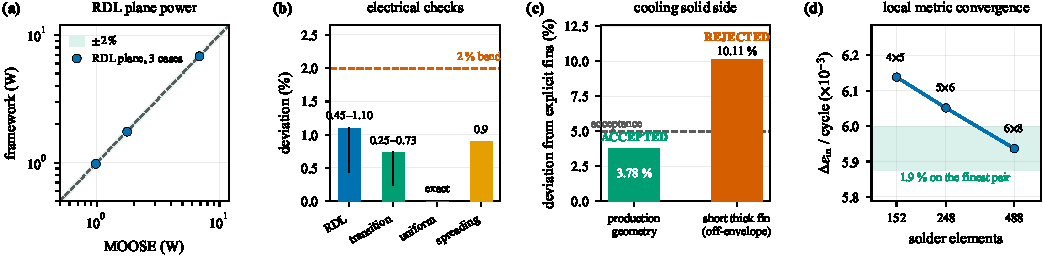
\includegraphics[width=\textwidth]{fig5_validation.pdf}
\caption{Validation. (a) Redistribution-plane dissipated power against MOOSE for three
regulator placements, and interconnect transition resistance for five geometries; all eight
within $1.2$\,\%. (b) Three-dimensional conduction against closed-form references, and the
measured land-spreading correction of the physical via chain. (c) Cooling solid side against
an explicitly meshed fin solution, with the rejected off-envelope geometry shown. (d) Mesh
refinement and cycle stabilisation of the local response metric.}
\label{fig:valid}
\end{figure*}

Four graded mesh levels bound the numerical uncertainty on the global warpage at $0.50$\,\%.
For the local submodel, three genuine mesh-refinement levels give a $1.9$\,\% change in the
per-cycle increment between the two finest, as shown in Fig.~\ref{fig:valid}(d); the
architecture \emph{ratio} is converged an order better because the residual error is largely
common mode. The per-cycle increment stabilises from $15.9$\,\% to $1.9$\,\% and then
$0.7$\,\% cycle-to-cycle, below the $5$\,\% criterion by the fourth cycle. An independent
integration route for the inelastic energy agrees to $0.79$--$1.56$\,\%.
Integration-tolerance sensitivity, measured separately on the frozen pair, is zero to twelve
digits across the tolerances that admit a solution, against $1.9$\,\% for the mesh.

\begin{table}[!t]
\caption{Validation matrix. Two attempts produced no usable result and are reported as such.}
\label{tab:valid}
\centering
\footnotesize
\setlength{\tabcolsep}{3.5pt}
\begin{tabular}{@{}L{2.30cm}L{1.50cm}L{1.45cm}L{2.05cm}@{}}
\toprule
Quantity & Production model & Reference & Error \\
\midrule
RDL plane power, 3 placements & sheet PDE & MOOSE, $300^{2}$ & $0.45$--$1.10$\,\% \\
Transition resistance, 5 geometries & analytic & MOOSE 3-D & $0.25$--$0.73$\,\% \\
Uniform conductor & finite volume & $\rho\ell/A$ & exact \\
Spreading resistance & finite volume & $\rho/(4a)$ & $+0.9$\,\% \\
Via-chain with lands & analytic series & finite volume & $1.16\times$, conv. $0.13$\,\% \\
Via AC ratio, 1\,MHz & skin-depth & Bessel & $\delta/r{=}4.41$, $1.0001$ \\
$k_{z}$, all layers & parallel rule & explicit RVE & $<1$\,\% \\
$k_{xy}$, bump field & Maxwell & explicit RVE & $<1.5$\,\% \\
$k_{xy}$, via array & explicit RVE & Maxwell & $11$--$39$\,\% high; RVE adopted \\
Cell periodicity & $1{\times}1$ & $2{\times}2$ & $0.000$\,\% \\
Cooling, fluid side & energy balance & closed form & exact \\
Cooling, solid side & fin efficiency & MOOSE, explicit fins & $3.78$\,\% \\
Loss decomposition & per-term & aggregate & machine precision \\
Heat deposition & per-layer & electrical total & $<10^{-6}$ rel. \\
Package thermal field & conduction & MOOSE 3-D & ordering preserved \\
PEEQ identity & CalculiX & creep-only test & $1.0000$ \\
Global warpage & 4 mesh levels & refinement & $0.50$\,\% \\
Local response & 3 mesh levels & refinement & $1.9$\,\% \\
Local integration tolerance & \textsc{cetol} $5{\times}10^{-2}$ & published case at the same tolerance & $0.0000$\,\% \\
Local response, frozen pair & 4 cycles & cycle-to-cycle & $0.04$, $0.06$\,\% \\
E--T fixed point & Picard & iterate difference & $<0.25$\,K, 3 iters \\
\midrule
Conjugate CFD & --- & ANSYS Icepak & discarded; \emph{not claimed} \\
Via loop AC, full wave & --- & ANSYS HFSS & did not converge; \emph{not claimed} \\
\bottomrule
\end{tabular}
\end{table}

The complete validation matrix, including the two attempts that produced no usable result,
is given in Table~\ref{tab:valid}.

% BEGIN final-lineage:matched
\subsection{Matched-reference benchmarks}\label{sec:matched}
Each production model was solved together with a reference on the same problem and the same
machine (Table~\ref{tab:accspeed}). Steady conduction $\nabla\!\cdot(k\nabla T)=0$ is the same
operator as $\nabla\!\cdot(\sigma\nabla V)=0$, so a commercial thermal finite-element solver
serves as the reference for the direct-current conduction stages under the exact analogy.
The single-via resistance agrees to \ErrTsvBulk\,\%, the residual being the faceted
representation of the circular section. The via-field homogenisation agrees to
\ErrTsvKz\,\% through thickness and \ErrTsvKx\,\% in plane. The redistribution-tier laminate
agrees to \ErrRdlKx\,\% in plane but overstates the through-thickness conductivity by
\ErrRdlKz\,\%, because the series form ignores constriction onto the copper grid; the
representative-volume values are therefore adopted and every thermal result uses them. The
package power network agrees with an open-source finite-element solution to
\ErrPkgRdlZone\,\% for Z1 and \ErrPkgRdlZtwo\,\% on the opening geometry of the BGA-fed control
on effective resistance; the direct-fed Z2 has no such network to check. For the package thermal solver, on the unit cell of each production stack (for Z2 the direct-fed stack with its explicit attach), a commercial finite-element solution of the same interior unit cell agrees with the production thermal solver to \ErrThermAedtZtwo\,\% (Z2) and \ErrThermAedtZone\,\% (Z1) of the temperature rise; an open-source finite-element solution on independent meshes agrees to \ErrThermMooseZone\,\% (Z1) and \ErrThermMooseZtwo\,\% (Z2), inside that reference's own mesh dependence. The cold-plate correlation that sets the top boundary was checked against a conjugate computational-fluid-dynamics solution of one microchannel half-pitch at the production heat load: the correlation overstates the mean base temperature rise by \ErrCoolingIcepak\,\%, so it is conservative, and halving the cross-section mesh moves the CFD value by less than 0.4\,\%. The correlation is not recalibrated to that solution: the coefficient that would reproduce the conjugate solution's mean base rise, \IcepakFactor\ times the compact one, is applied instead as a class-B sensitivity to both architectures; it changes the peak temperature by -2.7\,\% (Z1) and -2.6\,\% (Z2) and moves no ordering.
The thermoelastic element and its minimal supports reproduce the bimaterial closed form to \ErrMechClosed\,\%, the expected free-edge difference, and a commercial structural solution of the same bilayer to \ErrMechAedt\,\%. Runtimes are medians of three timed repeats after a warm-up on one machine; the
closed forms run in microseconds against minutes for the finite-element references, while
the finite-element-to-finite-element ratios compare solvers rather than model reduction.
These are model-specific comparisons on matched problems; no single framework accuracy is
defined, and no end-to-end speedup against a commercial flow is claimed.
% GENERATED by scripts/final_closure_manuscript_tables.py
\begin{table*}[!t]
\caption{Each production model against a matched reference on the same problem and machine. Runtimes are medians of three timed repeats after a warm-up (one solve per level for the conjugate CFD); the ratio is reference over production and is given only between field solvers, where it compares solvers, not model reduction. For a closed form, a homogenisation rule or the compact cooling correlation both runtimes are given and no ratio is printed. No single framework accuracy is defined and no end-to-end commercial speedup is claimed.}
\label{tab:accspeed}
\centering
\scriptsize
\begin{tabular}{@{}L{3.3cm}L{3.0cm}L{3.6cm}rrrr@{}}
\toprule
Stage & Production model & Reference & Error & Production & Reference & Ratio \\
\midrule
tsv bulk & rho L / A & AEDT Mechanical & -1.147\,\% & 0.6\,$\mu$s & 10.0\,s & -- \\
tsv tile kz & Voigt & AEDT Mechanical & +0.711\,\% & 0.7\,$\mu$s & 36.1\,s & -- \\
tsv tile kx & Maxwell-Garnett & AEDT Mechanical & +0.255\,\% & 0.8\,$\mu$s & 36.0\,s & -- \\
rdl tier kx & laminate, grid in-plane & AEDT Mechanical & -3.694\,\% & 0.6\,$\mu$s & 34.1\,s & -- \\
rdl tier kz & laminate, series & AEDT Mechanical & +12.490\,\% & 1.3\,$\mu$s & 34.1\,s & -- \\
pkg 48 V RDL, Z1 & voltage-fed aligned graded FV sheet (L3) & MOOSE & +0.079\,\% & 15.8\,s & 55.0\,s & 3.47$\times$ \\
pkg 48 V RDL, Z2 control & voltage-fed aligned graded FV sheet (L3) & MOOSE & +0.108\,\% & 24.4\,s & 60.8\,s & 2.49$\times$ \\
thermal column aedt Z1 & CalculiX C3D8 structured hex & AEDT Mechanical & -0.141\,\% & 70.7\,s & 154.7\,s & 2.19$\times$ \\
thermal column moose Z1 & CalculiX C3D8 structured hex & MOOSE & -0.163\,\% & 67.2\,s & 28.7\,s & 0.43$\times$ \\
thermal column aedt Z2 & CalculiX C3D8 structured hex & AEDT Mechanical & -0.111\,\% & 41.9\,s & 126.9\,s & 3.03$\times$ \\
thermal column moose Z2 & CalculiX C3D8 structured hex & MOOSE & -0.125\,\% & 42.7\,s & 28.2\,s & 0.66$\times$ \\
mech bilayer closed form & CalculiX C3D8I & Timoshenko bimaterial curvature & -0.433\,\% & 65.9\,s & -- & -- \\
mech bilayer aedt & CalculiX C3D8I & AEDT Mechanical & +0.014\,\% & 65.9\,s & 262.7\,s & 3.99$\times$ \\
structural solver iterative vs direct & CalculiX ITERATIVE CHOLESKY & CalculiX SPOOLES (direct) & -0.010\,\% & -- & -- & -- \\
cooling icepak & laminar microchannel correlation (Shah \& London Nu, fin efficiency, caloric + base resistance) & Ansys Icepak 2026 R1 conjugate CFD & +16.484\,\% & 12.1\,$\mu$s & 1305.4\,s & -- \\
\bottomrule
\end{tabular}
\end{table*}

% END final-lineage:matched
\subsection{Computational cost}
\begin{table}[!t]
\caption{Measured computational cost of one evaluation of the historical frozen pair. The timing run reproduced the frozen results exactly.}
\label{tab:cost}
\centering
\footnotesize
\begin{tabular}{@{}p{3.1cm}p{2.1cm}rc@{}}
\toprule
Stage & Size & Wall time & Threads \\
\midrule
Converter synthesis & 90-device library & $4.56$\,s & 1 \\
Rail-aware PPDN + routing & 6 segments $\times$ 49 cells & $0.10$\,ms & 1 \\
Cooling correlation & 223 channels & $11.2$\,ms & 1 \\
Full ETM evaluation, Z1 & 3 E--T iterations & $134.6$\,s & 48 \\
Full ETM evaluation, Z2 & 3 E--T iterations & $204.2$\,s & 48 \\
\midrule
\multicolumn{4}{@{}p{7.6cm}}{\footnotesize Platform: 2$\times$Intel Xeon Gold 6342 @ 2.80\,GHz,
48 physical cores, 2.0\,TiB, RHEL 8.10, CalculiX 2.23, Python 3.12.14. No accelerator.
Historical evaluation; stage-level runtimes of the physical lineage against matched
references are given in Table~\ref{tab:accspeed}.}\\
\bottomrule
\end{tabular}
\end{table}

Table~\ref{tab:cost} reports the measured cost of one complete evaluation of the historical frozen pair, which fixes the cost structure of the framework. The timing run
reproduced the frozen results exactly, so the times correspond to the evaluation that
produced the reported numbers.

The analytical layers are effectively free relative to the finite-element solves. Converter
synthesis over the 90-device library costs $4.56$\,s once; the per-design rail-aware network
evaluation costs $0.10$\,ms and the cooling correlation $11.2$\,ms. A complete
electrothermal--mechanical evaluation costs $134.6$\,s for the embedded architecture and
$204.2$\,s for the backside architecture. The split follows the execution path rather than
the loop count. Each fixed-point iteration contains thermal finite-element work only, and the
thermal solve is itself fluid-coupled, so each iteration runs three to four thermal
sub-solves: eleven in total over the three iterations, $75.1$\,s for the embedded and
$121.4$\,s for the backside architecture. The thermoelastic solve is \emph{not} inside the
loop. It is entered once, after the temperature field has converged, for $49.5$\,s and
$67.6$\,s respectively, which is the one-way thermal-to-mechanical coupling of
Section~\ref{sec:thermech}. The local solder submodel is a further $45.0$\,s and $35.1$\,s,
entered once per architecture. The remainder is mesh construction, material assembly, input
writing and result parsing. The two architectures differ because the backside stack resolves
a through-substrate via field the embedded stack does not, changing the element count; both
converge in three iterations.

This cost structure is the practical argument for the framework's organisation: the numerical
work is confined to the thermal solves inside the loop, one thermoelastic solve after it and
one local submodel, and everything that can be evaluated in closed form is, so that the
expensive part is entered once per candidate rather than once per design variable.

% BEGIN final-lineage:cost
On the physical lineage, one converged electrothermal fixed point costs \EtWallZone\,s (Z1)
and \EtWallZtwo\,s (Z2) on the production grid, and the single thermoelastic solve that
follows it \MechWallZone\,s and \MechWallZtwo\,s, on the same machine. Stage-level runtimes
of each production model against its matched reference are reported with the accuracy
comparison in Table~\ref{tab:accspeed}. No end-to-end speedup against a commercial flow is
claimed, because no commercial flow evaluates the same coupled problem.
% END final-lineage:cost

\section{Comparison With Existing DVPD Frameworks}\label{sec:compare}

\subsection{Capability comparison}
\begin{table*}[!t]
\caption{Capability comparison with DVPD and package co-design frameworks whose full text was examined. \checkmark: modelled explicitly; $\triangle$: partial, assumed, or reported as future work; ---: not included. Rows below the rule are capabilities the present framework does not provide.}
\label{tab:cmp}
\centering
\footnotesize
\setlength{\tabcolsep}{4pt}
\begin{tabular}{@{}lccccccc@{}}
\toprule
Capability & \cite{Krishnakumar2026DVPD} & \cite{Sriharini_ECTC_24} & \cite{ISCAS2024DVPD} & \cite{VPD2023Architectures} & \cite{DVPD2026PowerMgmt} & \cite{Wang2025TTSV} & This work \\
\midrule
Converter synthesis from a device library & \checkmark & \checkmark & \checkmark & $\triangle$ & --- & --- & \checkmark \\
Multi-stage hybrid regulator topology & \checkmark & \checkmark & \checkmark & \checkmark & $\triangle$ & --- & \checkmark \\
Switching, gate and $C_{\mathrm{oss}}$ loss terms & \checkmark & $\triangle$ & $\triangle$ & $\triangle$ & \checkmark & --- & \checkmark \\
Rail-aware per-segment current assignment & $\triangle$ & $\triangle$ & $\triangle$ & $\triangle$ & $\triangle$ & --- & \checkmark \\
Geometry-derived through-substrate via model & \checkmark & \checkmark & $\triangle$ & $\triangle$ & --- & \checkmark & \checkmark \\
Geometry-derived RDL plane model & \checkmark & \checkmark & \checkmark & $\triangle$ & \checkmark & \checkmark & \checkmark \\
Bump and transition resistance & $\triangle$ & \checkmark & --- & \checkmark & --- & $\triangle$ & \checkmark \\
Intra-converter routing inside the cell & --- & --- & --- & --- & \checkmark & --- & \checkmark \\
Temperature-dependent $\rho$ and $R_{\mathrm{on}}$ & \checkmark & --- & --- & --- & --- & \checkmark & \checkmark \\
Component heights in the stack budget & $\triangle$ & --- & --- & $\triangle$ & --- & --- & \checkmark \\
Component partition across tiers & $\triangle$ & --- & --- & \checkmark & --- & --- & \checkmark \\
Electrical--thermal fixed point & \checkmark & --- & $\triangle$ & --- & --- & \checkmark & \checkmark \\
Anisotropic / homogenised thermal model & $\triangle$ & --- & --- & --- & --- & \checkmark & \checkmark \\
Physical cooling boundary with a stated domain & \checkmark & --- & $\triangle$ & --- & --- & \checkmark & \checkmark \\
Pump power separated from electronics scope & $\triangle$ & --- & --- & --- & --- & --- & \checkmark \\
Global thermoelastic package model & --- & --- & --- & --- & --- & --- & \checkmark \\
Explicit assembly state, free against mounted & --- & --- & --- & --- & --- & --- & \checkmark \\
Local solder inelastic-response model & --- & --- & --- & --- & --- & --- & \checkmark \\
Mechanical-to-electrical feedback quantified & --- & --- & --- & --- & --- & --- & \checkmark \\
Vertical-interconnect realizability check & --- & --- & --- & $\triangle$ & --- & $\triangle$ & \checkmark \\
Manufacturability separated from feasibility & --- & --- & --- & --- & --- & $\triangle$ & \checkmark \\
Independent cross-solver validation reported & $\triangle$ & --- & $\triangle$ & --- & --- & \checkmark & \checkmark \\
Computational cost reported & --- & --- & --- & --- & --- & $\triangle$ & \checkmark \\
\midrule
Load-dependent operating point & --- & --- & --- & --- & \checkmark & --- & --- \\
Regulator activation and power management & --- & --- & --- & --- & \checkmark & --- & --- \\
Output ripple and regulation constraint & $\triangle$ & $\triangle$ & $\triangle$ & $\triangle$ & \checkmark & --- & $\triangle$ \\
Manufacturing-cost objective & --- & --- & --- & --- & --- & \checkmark & --- \\
\bottomrule
\end{tabular}
\end{table*}

Table~\ref{tab:cmp} compares the framework with five DVPD studies and one 2.5-D
electrothermal co-optimization study. Only works whose full text was examined are scored;
capability is not inferred from a title or an abstract, and several relevant works could not
be obtained in full text from the present host and are consequently cited for motivation but
left unscored.

The comparison is not a deficiency list, and the rows below the rule are capabilities the
present framework does not have. The architecture study~\cite{VPD2023Architectures} defines
the vertical-integration family used here---power devices on the interposer periphery, power
devices embedded beneath the die, and multi-stage variants---and establishes the 1\,kW,
high-current-density operating point; the embedded and backside alternatives evaluated in
this work are two members of that family. The baseline design
framework~\cite{Krishnakumar2026DVPD} co-optimises converter synthesis, interconnect
allocation and floorplanning under thermal feasibility, and it identifies multi-substrate
vertical stacking and chiplet embedding as the enabling packaging technologies; the present
work takes that identification as its starting point and asks what the package does to the
architecture ranking once those technologies are represented geometrically. The power-management
methodology~\cite{DVPD2026PowerMgmt} resolves conduction loss by routing segment, including
the path inside the regulator cell, and adds a capability absent here: the operating point is
load-dependent, regulators are activated according to instantaneous demand, and ripple and
regulation are constrained explicitly. The present framework evaluates a single full-load
operating point and does not model activation, so its loss figures are not comparable with a
light-load result. The 2.5-D study~\cite{Wang2025TTSV} carries a manufacturing-cost objective
and reports validation errors of $3.97$\,\% on impedance and $0.35$\,\% on temperature, but
contains no converter synthesis and no mechanical model. The distinguishing rows for the
present work are intra-converter routing geometry, component partition across tiers, assembly
state, local solder response and the separation of manufacturability from feasibility.

\subsection{Reproduction and testing of published positions}
\begin{table*}[!t]
\caption{Positions from the prior DVPD literature, reproduced within the framework and tested.
Each is labelled by its standing in the cited work: a \emph{published result} is stated there
explicitly, an \emph{implication of the formulation} follows from how that work is set up
without being claimed, and a \emph{modelling assumption} is a choice the cited model makes.
The purpose is to identify the conditions under which each holds.}
\label{tab:prior}
\centering
\scriptsize
\setlength{\tabcolsep}{4pt}
\begin{tabular}{@{}p{4.5cm}p{3.9cm}p{3.7cm}p{4.5cm}@{}}
\toprule
Position, and its standing in the cited work & Representation here & Outcome & Interpretation \\
\midrule
\emph{Published result.} Vertical interconnect loss is small relative to lateral routing; the
loss breakdown is reported and vertical dissipation called negligible
\cite{VPD2023Architectures,Krishnakumar2026DVPD,Sriharini_ECTC_24,ISCAS2024DVPD}
& each vertical segment carries its assigned rail; loss from via geometry and segment current
& \textbf{reproduced, and rail-dependent}: the identical field dissipates $\approx0$\,W carrying 48\,V and $0.991$\,W carrying 1\,V
& holds for a high-voltage vertical path; does not transfer to a low-voltage one \\
\emph{Published result.} Lateral delivery of the low-voltage rail dominates delivery loss, and
is the stated motivation for converting near the load
\cite{VPD2023Architectures,Krishnakumar2026DVPD,Sriharini_ECTC_24,ISCAS2024DVPD}
& same sheet model, geometry-derived width, $\rho(T)$
& \textbf{reproduced}
& retained as motivation; no general claim about 2.5-D delivery is made \\
\emph{Implication of the formulation}, not an explicit conclusion: a larger converter footprint
is favourable, since it lowers current density and loss in the cited flows
\cite{Krishnakumar2026DVPD,ISCAS2024DVPD}
& same variation, evaluated free and on five explicit boards
& \textbf{reversed by assembly state}: warpage $+20.3$\,\% free, $-16.6$ to $-29.0$\,\% mounted
& the electrical preference is unchanged; a free-package mechanical screen inverts the sign \\
\emph{Implication of the formulation}: substrate thickness is selected on electrical and thermal
grounds, no mechanical model being present \cite{Krishnakumar2026DVPD,Sriharini_ECTC_24}
& same variation through the thermoelastic model under the explicit assembly
& \textbf{no opposition found} in the evaluated range
& thickness remains an electrical--thermal decision here \\
\emph{Implication of the formulation}: tier assignment is treated as electrically free, counts,
area and height being unchanged by it \cite{Krishnakumar2026DVPD,VPD2023Architectures}
& assignment propagated into the conductor-plane topology; per-net aspect ratio and landing area checked
& \textbf{invalidated for one ordering}: worst aspect ratio $5.05$ against $0.833$
& tier assignment is constrained by package conductor-plane structure, invisibly to an electrical model \\
\emph{Modelling assumption}: peak temperature is the thermal figure carried into feasibility or
the objective, and no local mechanical response is evaluated alongside it
\cite{Krishnakumar2026DVPD,ISCAS2024DVPD,Wang2025TTSV}
& $T_{\max}$ and local corner-joint response on the same converged field
& \textbf{not equivalent} on the frozen pair: $+8.14$\,K against $-18.4$\,\% inelastic response (conditional, Sec.~\ref{sec:backside-limit})
& $T_{\max}$ is insufficient to rank local mechanical response; a counterexample suffices, and temperature remains inside the response model \\
\bottomrule
\end{tabular}
\end{table*}

Six positions taken in this literature were reproduced within the framework and tested. The
purpose is to identify the conditions under which each holds, not to contest it. Two of the
six are results the cited works state explicitly; the remaining four are not claimed there in
those words, and are labelled in Table~\ref{tab:prior} as implications of how those flows are
formulated or as modelling assumptions they make. They are tested as such. The results are
summarised in Table~\ref{tab:prior} and three are developed below.

\emph{Vertical interconnect loss is small.} This is reproduced and found to be
rail-dependent. The through-substrate field is geometrically identical in both
architectures, but in the embedded case it carries the 48\,V input rail and dissipates
essentially nothing, while in the backside case it carries the 1\,V output rail at the full
cell current and dissipates $0.991$\,W, as shown in Fig.~\ref{fig:loss}(c). The conclusion
holds for a high-voltage vertical path and does not transfer to a low-voltage one. Vertical
loss is a property of the rail assignment rather than of the interconnect, which is why the
model assigns rails per segment.

\begin{figure*}[!t]
\centering
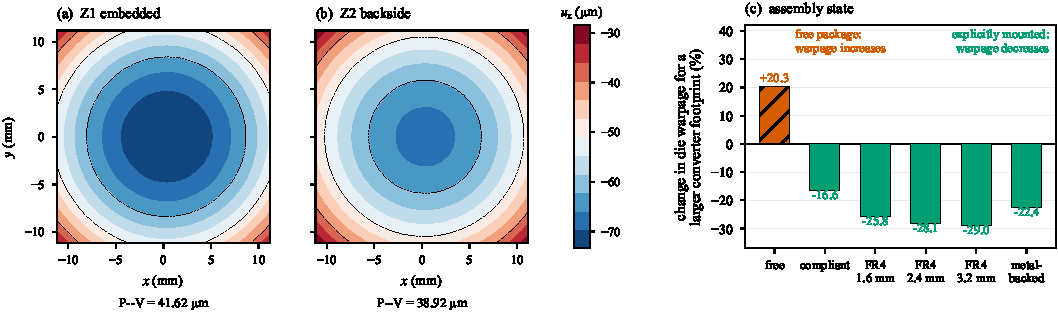
\includegraphics[width=\textwidth]{fig6_assembly.pdf}
\caption{Package deformation and assembly state. (a), (b) Out-of-plane displacement of the
die surface for the frozen pair, on one shared scale, from the converged thermoelastic solve
of Section~\ref{sec:thermech}, drawn on the $30\times30$ die-surface nodes of the global
mesh; both surfaces are domed, and the embedded architecture carries the larger
peak-to-valley. (c) Change in die warpage when the converter footprint is
enlarged, evaluated for the free package and for five explicit board constructions. The sign
of the interaction reverses between the free and the mounted state, so a mechanical
conclusion obtained in one state cannot be quoted in the other.}
\label{fig:assembly}
\end{figure*}

\emph{A larger converter footprint is favourable.} This is reproduced electrically and
thermally, and it reverses mechanically with the assembly state. Fig.~\ref{fig:assembly}
reports the change in die warpage when the converter footprint is enlarged: for the free
package the warpage increases by $20.3$\,\%, and on each of five explicit board
constructions spanning compliant to metal-backed it decreases, by between $16.6$ and
$29.0$\,\%. The electrical preference is unchanged; the mechanical consequence changes sign.
A free-package mechanical screen can therefore invert the conclusion it is used to support.

\emph{Component tiers may be assigned on electrical grounds.} This is invalidated for one
ordering by physical realizability. Two tier orderings of the same components, identical in component count, per-tier area and total stack height, and therefore
equivalent at the component-selection and stack-budget level, differ by a factor of six in
the worst via aspect ratio their vertical nets require. They are not identical electrically:
each order fixes which rail crosses which dielectric depth, so the intra-cell routing
parasitics differ between them. That difference is carried inside the final refinement step
of Table~\ref{tab:ablation} together with the conductor-plane correction, and is not
separated from it here. The mechanism is developed in Section~\ref{sec:arch}.

\section{Cross-Domain Architecture Study}\label{sec:arch}
% BEGIN final-lineage:arch-frame
The sensitivity, robustness and repartition studies of this section were carried out on the
historical frozen representation of the two architectures. They establish how the response
depends on the design variables, but their architecture ordering is superseded by the
physical lineage of Sec.~\ref{sec:physical}, which reverses the mechanical ordering.
% END final-lineage:arch-frame

\subsection{Sensitivity of the mechanical response to DVPD variables}
Of the converter-level variables, the number of regulator cells is mechanically inert over
the swept range: redistributing the same total dissipation over more or fewer cells does not
materially change the corner-joint response. The variables that matter are geometric---
substrate thickness, tier partition and the resulting stiffness distribution---consistent
with deformation being driven by the mismatch of the stack rather than by the granularity of
the heat source.

Global die warpage and the local corner-joint driver track in direction but not in
magnitude. In the frozen pair the architecture with the larger die warpage carries the larger
local driver, so the direction is consistent; the warpage differs by $6.5$\,\%, the
corner-joint driver $\du$ by $16.3$\,\% and the local inelastic response
$\Delta\varepsilon_{\mathrm{in}}$ by $18.4$\,\%. Global warpage is therefore a useful screen and an
insufficient reliability metric on its own.

\subsection{Robustness of the architecture ordering}
\begin{figure}[!t]
\centering
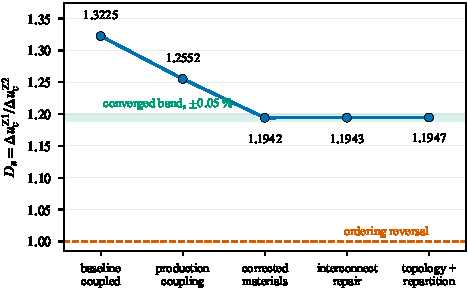
\includegraphics[width=\columnwidth]{fig7_sensitivity.pdf}
\caption{Displacement-driver ratio $D_{u}$ under successive refinement of the physical
model. The ratio
converges as the geometric representation is corrected and is thereafter insensitive; the
architecture ordering is preserved at every stage.}
\label{fig:sens}
\end{figure}

The quantity tracked through the refinement sequence is the ratio of the
corner-joint displacement drivers,
$D_{u} = \Delta u_{\mathrm{c}}^{\mathrm{Z1}} / \Delta u_{\mathrm{c}}^{\mathrm{Z2}}$.
Fig.~\ref{fig:sens} reports $D_{u}$ as the physical representation was successively refined:
from an initial coupled model, through production-level coupling, corrected package
materials and architecture-aware via spans, an interconnect repair, and finally the
conductor-plane topology and component repartition described below. The ratio falls from
$1.3225$ to $1.1942$ as the geometry is corrected and is thereafter insensitive, the last
three refinements moving it by less than $0.05$\,\% in total. The ordering is never in
question and the magnitude converges. This separation---a robust ordering with a magnitude
that remains model-dependent until the geometry is physical---is why the ordering is reported
as a result and the magnitude as an envelope.

\subsection{Component repartition}
In the reference tier order---high-side switch, low-side switch, flying capacitors, then
inductor and output capacitor---the switch-node connection must cross the flying-capacitor
tier, and the connection between the high-side device and the flying capacitors must cross
the entire low-side tier. The latter is the demanding one: a $606$\,\textmu m crossing implies
a build-up via of aspect ratio $5.05$ at the frozen low-side height, $5.32$ at the selected
one, at the finest pitch reported for a comparable
embedded-die process~\cite{Ostmann2008ChipEmbedding}, well outside routine microvia
practice~\cite{Cauwe2023HDI}.

All assignments of the existing components to tiers were enumerated subject to the per-tier
area budget and scored by the dielectric depth each high-current net must cross. Of 144
assignments satisfying the area budget, eight retain both endpoints fixed by the reference
architecture---the high-side device flip-chipped at the bottom substrate and the inductors in
the top tier adjacent to the points of load. The preferred assignment exchanges the low-side
switches with the flying capacitors and changes nothing else. It is a permutation: the same
component classes, the same counts, the same per-tier areas and the same stack height
($1921$\,\textmu m at the frozen device heights, $1953$\,\textmu m at the selected ones), so
every area and height result carries over unchanged.

The effect on the vertical interconnect is substantial. The switch node becomes an
adjacent-tier transition through a single redistribution layer, the high-side to
flying-capacitor connection becomes adjacent as well, and the only remaining build-up via
carries $1.435$\,A. The worst aspect ratio over all vertical nets falls from $5.05$ to
$0.833$ and the worst ratio of required to available vias is $0.633$, as shown in
Fig.~\ref{fig:realize}.

% BEGIN final-lineage:physical
\subsection{Physical architecture comparison}\label{sec:physical}
The physical lineage is evaluated for both architectures---Z1 and the direct-fed Z2---in every named 48\,V scenario
(Table~\ref{tab:physical}); the electrothermal fixed point converges within \EtIters\
iterations in every case. In the continuous-input scenario the two architectures dissipate, each inside its package-internal boundary,
\PlossZone\,W (Z1) and \PlossZtwo\,W (Z2) and reach \TmaxZone\ and \TmaxZtwo\,$^\circ$C. The
critical joint, found by evaluating the in-plane relative displacement across the ball layer
at every legal site (\NjointZone\ for Z1 and \NjointZtwo\ for Z2) rather than assumed, is the
outermost lattice corner in both. There the backside architecture carries a joint
displacement driver of \DuZtwo\,$\mu$m against \DuZone\,$\mu$m, a local inelastic strain
increment per stabilised cycle of \EpsZtwo\ against \EpsZone, and a die warpage of
\WarpZtwo\ against \WarpZone\,$\mu$m. The embedded architecture carries the lower die warpage and joint displacement driver in every scenario that admits a valid comparison. Electrically, the backside architecture dissipates less inside the package in every scenario that admits a valid comparison. The platform-inclusive loss has no unconditional winner: in HV-S0 Z2 has the lower platform-inclusive loss only while the complete direct-feed loop stays below $R^{*}$ = 1.77\,m$\Omega$, and Z1 above it; in HV-S1 Z2 has the lower platform-inclusive loss only while the complete direct-feed loop stays below $R^{*}$ = 3.76\,m$\Omega$, and Z1 above it; HV-S2 is not rankable (the Z1 operating point is inadmissible). No value of that loop resistance is known, so no platform-level ranking is claimed.
Thermally, the embedded architecture runs cooler in the continuous-input scenario, the backside architecture runs cooler in the buck-duty pulse---the peak-temperature ordering reverses with the scenario. Under the overall-ratio pulse the embedded operating point leaves the valid solid-solder domain under the assumed cooling; that scenario is an infeasibility result, and no architecture ordering of any quantity is drawn there. Peak temperature therefore does not rank the local mechanical response on
the physically closed pair either. The frozen pair of Sec.~\ref{sec:histrep} showed the opposite mechanical ordering; the physical closure reverses it. Fig.~\ref{fig:physical} shows the per-scenario
results, the joint driver at every legal site and the matched-reference errors.
\begin{figure*}[!t]
\centering
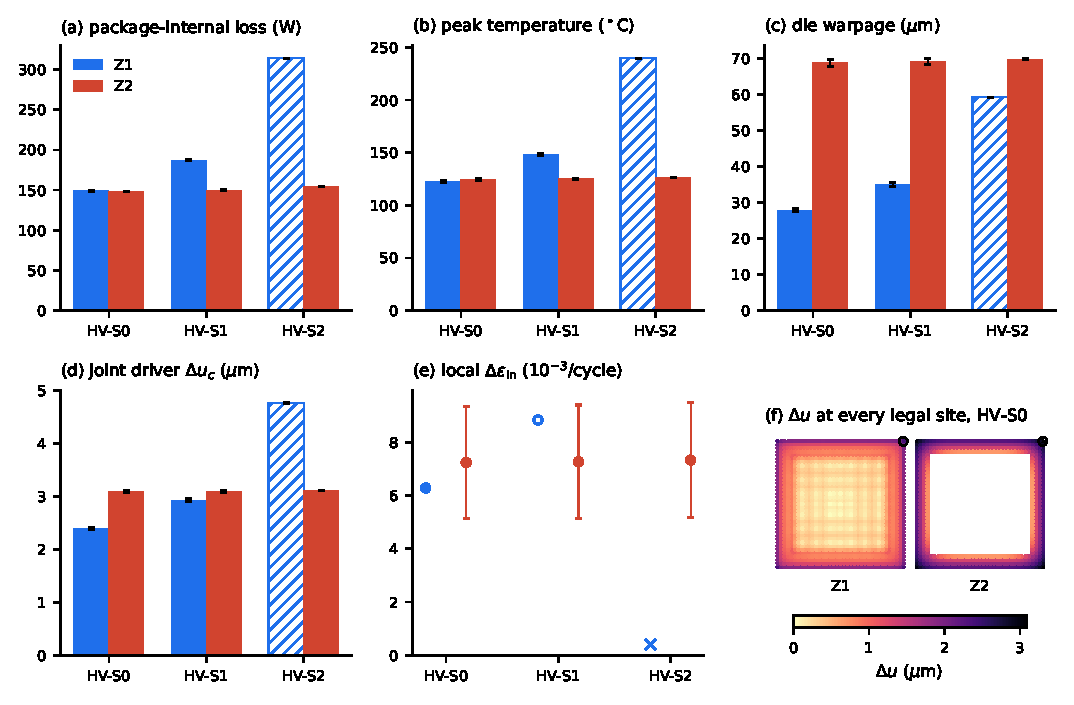
\includegraphics[width=\textwidth]{fig9_physical.pdf}
\caption{Physical lineage on the production mesh, one quantity per panel: (a) loss, (b) peak
temperature, (c) die warpage, (d) critical-joint displacement driver, per named scenario, with
whiskers at the measured discretisation uncertainty (hatched: critical joint at or above the
solder melting onset, an infeasibility result shown but not ranked); (e) local inelastic strain per cycle on the
production local mesh with its uncertainty $U$ (open marker: joint beyond the constitutive
calibration, extrapolated; cross: joint at or above the solder melting onset, no valid
response); (f) in-plane joint displacement driver at every legal ball site in the
continuous-input scenario, critical joint circled. Matched-reference errors and runtimes are in
Table~\ref{tab:accspeed}.}
\label{fig:physical}
\end{figure*}
% GENERATED by scripts/final_closure_manuscript_tables.py
\begin{table}[!t]
\caption{Physical lineage: converged results per named 48\,V scenario (HV-S0/S1/S2 are named scenarios, not a bracket). Matched BGA count 54 per rail; production mesh: graded $h_{xy}$ = 1.1 mm grid, every in-plane interval split in 2. $\Delta\varepsilon_{\mathrm{in}}$ is the inelastic strain increment per stabilised cycle; no life is derived from it.}
\label{tab:physical}
\centering
\footnotesize
\setlength{\tabcolsep}{2.5pt}
\begin{tabular}{@{}llrrrrr@{}}
\toprule
Scen. & Arch. & $P_{\mathrm{loss}}$ (W) & $T_{\max}$ ($^\circ$C) & warp ($\mu$m) & $\du$ ($\mu$m) & $\Delta\varepsilon_{\mathrm{in}}$ \\
\midrule
HV-S0 & Z1 & 146.47 & 121.58 & 27.64 & 2.374 & $6.485\times10^{-3}${} \\
HV-S0 & Z2 & 142.67 & 120.59 & 69.28 & 3.951 & $1.118\times10^{-2}${} \\
HV-S1 & Z1 & 185.86 & 147.95 & 34.86 & 2.921 & $9.135\times10^{-3}${}$^\dagger$ \\
HV-S1 & Z2 & 165.51 & 124.59 & 72.96 & 4.272 & $1.274\times10^{-2}${} \\
HV-S2 & Z1 & 322.92 & 243.39 & 60.18 & 4.841 & \emph{n.c.}{}$^\dagger$$^\ddagger$ \\
HV-S2 & Z2 & 223.81 & 137.71 & 82.34 & 5.094 & $1.616\times10^{-2}${}$^\dagger$ \\
\bottomrule
\end{tabular}
\par\smallskip\raggedright $^\dagger$joint temperature above the 125\,$^\circ$C calibration of the Norton card (extrapolation); $^\ddagger$joint at or above the SAC305 melting onset (about 217\,$^\circ$C), not an admissible operating point. n.c.: no converged local response at that operating point.
\end{table}

% END final-lineage:physical
% BEGIN final-lineage:crossover
\subsubsection{Direct-feed requirement}\label{sec:crossover}
\begin{figure}[!t]
\centering
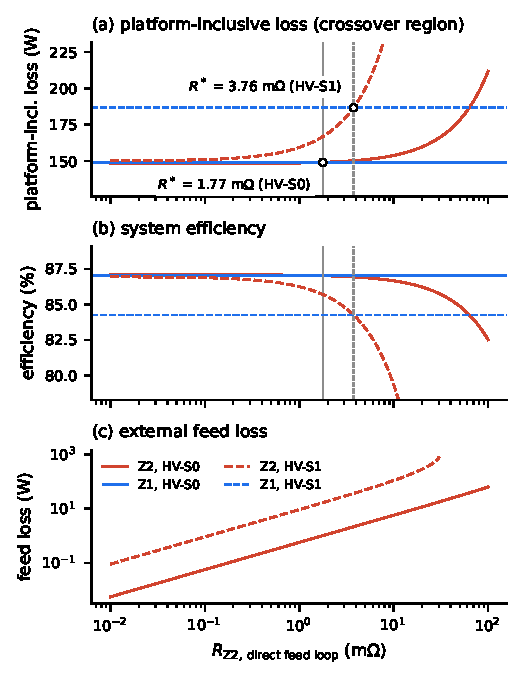
\includegraphics[width=\columnwidth]{fig10_crossover.pdf}
\caption{Direct-feed crossover. Z2 total loss (a), system efficiency (b) and external feed loss
(c) against the swept loop resistance $R_{\mathrm{Z2,feed}}$ of \eqref{eq:feed}; Z1's converged
package-internal loss and efficiency are the horizontal references. Open marker: $R^{*}$, where
the two losses are equal. A scenario in which the embedded operating point is inadmissible has no
valid reference and is not drawn.}
\label{fig:crossover}
\end{figure}
In the continuous-input scenario the package-internal losses are \PlossZone\,W (Z1) and \PlossZtwo\,W (Z2); at $I_{48,\mathrm{rms}} = \IrmsSzero$\,A each milliohm of external loop dissipates a further \PfeedPerMohmSzero\,W in Z2. Z2's advantage of \AdvZeroFeedSzero\,W with a lossless feed is gone at $R^{*} = \RstarSzero$\,m$\Omega$, where the feed dissipates \PfeedRstarSzero\,W. Under the buck-duty pulse the input RMS current is \IrmsSone\,A and Z1's own package 48\,V path grows with its square, so Z2 is ahead by \AdvZeroFeedSone\,W with a lossless feed and keeps that advantage up to $R^{*} = \RstarSone$\,m$\Omega$. Under the overall-ratio pulse the embedded operating point is inadmissible, so no crossover is defined there. For Z2 to preserve its electrical advantage, the direct-feed loop resistance must remain below \RstarSzero\,m$\Omega$ under the continuous-input scenario and below \RstarSone\,m$\Omega$ under the buck-duty pulse (Fig.~\ref{fig:crossover}). This is a requirement on the connector, its cable or bus and its contacts, including the distribution to the 49 input terminals; no source available to this work gives such a loop resistance, so whether it is met is not claimed. Depositing the feed loss at the largest loop resistance any requirement admits, at the continuous-input current, inside the package in the deepest converter tier---the worst place it could land---changes the Z2 peak temperature by +0.7\,\%, its die warpage by +0.8\,\% and its joint driver by +0.4\,\%, and moves the package-internal loss verdict.
% END final-lineage:crossover
% BEGIN final-lineage:control
\subsubsection{Controlled BGA-fed experiment}\label{sec:control}
This controlled experiment isolates the effect of BGA placement and the opening when both
architectures are forced to use an identical package-level 48\,V feed; it is not the primary Z2
construction. On the same corrected geometry---explicit attach, open sidewall clearance---the
BGA-fed control dissipates \PlossCtrl\,W, \CtrlMinusZtwo\,W more than the direct-fed Z2, of which
\CtrlPkgHV\,W are its package 48\,V RDL and ball terms (Table~\ref{tab:ledger}); it reaches
\TmaxCtrl\,$^\circ$C, a die warpage of \WarpCtrl\,$\mu$m and a joint driver of \DuCtrl\,$\mu$m. Its mechanical response differs from the direct-fed Z2 by +0.3\,\% in die warpage and +0.8\,\% in joint driver, so the feed choice is electrical: the opening and the ball placement, not the 48\,V path, set the mechanics. Z1, which uses the same package feed, dissipates \PlossZone\,W. The
control places its 48\,V input at the
high-side redistribution tier, as Z1 and the direct-fed Z2 do, although its feed arrives at the
land-side tier; the roughly 1.3\,mm traverse between the two is not modelled, so the control
understates its own loss slightly. The defect affects the control only.
% END final-lineage:control
% BEGIN final-lineage:localmesh
\subsubsection{Local solder discretisation}\label{sec:localmesh}
The local response is computed on a declared family of four solder meshes at each production
critical joint (L0 to L3; L3 halves every L0 interval in plane and through the solder), and the
rule that classifies it was declared before the finer levels were read: converged if the change
between the two finest levels is below 2\,\%, otherwise bounded by Richardson extrapolation
over the three finest levels, or by their range if the sequence is not monotone. Three
amendments to the procedure were needed, each declared before the results it governs. The
solver will not cut a time increment below $10^{-6}$ of the step period, which blocked the
cutbacks the finest meshes need at a load reversal; a first change made to work around it failed
its own acceptance test, the published harness control moving by $10.2\,\%$. The cause was a
post-processing defect, not the time integration: the solver prints output times to seven
significant digits, increments shorter than about 1\,ms at a load step print the same time as
the step boundary, and the time-keyed parser averaged them, biasing only the last cycle---the
reported one. An extraction that keeps every increment in file order reproduces the published
control to all ten printed digits, leaves every earlier production value unchanged, and puts
the first-increment sensitivity below \UtimeMax\,\% and the change from 4 to 16 cycles below
\UcycMax\,\%. Writing each load change as its own 3\,s step lifts the increment floor
without changing the load history and completes the finest level in every case.
Table~\ref{tab:localmesh} gives the response on every level, the rule outcome and the
uncertainty $U = U_{\mathrm{mesh}} + U_{\mathrm{time}} + U_{\mathrm{cyc}}$; \LocalNconverged\
of the \LocalNcases\ policy cases converge, and the local response is therefore reported as
\LocalMeshPhrase. A local ordering is drawn only where the Z1/Z2 gap exceeds twice the larger
$U$ of the pair. No local inelastic response ranking can be drawn. In HV-S0 the difference lies within the measured discretisation uncertainty, so no ranking is drawn. In HV-S1 the difference lies within the measured discretisation uncertainty (and the Z1 response is extrapolated), so no ranking is drawn. HV-S2 is not rankable because the Z1 operating point is physically inadmissible for the solid-solder model.
% GENERATED by scripts/final_closure_manuscript_tables.py
\begin{table}[!t]
\caption{Local solder discretisation under the declared policy: the response $\Delta\varepsilon_{\mathrm{in}}$ ($\times10^{-3}$ per cycle) on each level, the rule outcome and the uncertainty carried into the ordering, $U = U_{\mathrm{mesh}} + U_{\mathrm{time}} + U_{\mathrm{cyc}}$ (\%); conv.: converged (rule A), bound.: bounded (Richardson, rule B).}
\label{tab:localmesh}
\centering
\footnotesize
\setlength{\tabcolsep}{2.2pt}
\begin{tabular}{@{}lrrrrlrrrr@{}}
\toprule
Case & L0 & L1 & L2 & L3 & status & $U_{\mathrm{m}}$ & $U_{\mathrm{t}}$ & $U_{\mathrm{c}}$ & $U$ \\
\midrule
Z1 S0 & 6.487 & 6.359 & 6.277 & 6.203 & conv. & 1.19 & 0.02 & 0.82 & 2.03 \\
Z2 S0 & 11.186 & 10.572 & 10.212 & 9.971 & bound. & 18.11 & 0.03 & 0.10 & 18.23 \\
Z1 S1 & 9.137 & 8.994 & 8.893 & 8.793 & conv. & 1.14 & 0.03 & 0.41 & 1.57 \\
Z2 S1 & 12.737 & 12.109 & 11.712 & 11.449 & bound. & 15.51 & 0.03 & 0.08 & 15.63 \\
Z2 S2 & 16.166 & 15.489 & 15.039 & 14.715 & bound. & 27.88 & 0.02 & 0.05 & 27.95 \\
\bottomrule
\end{tabular}
\end{table}

% END final-lineage:localmesh
% BEGIN final-lineage:sens
\subsubsection{Sensitivity of the orderings}\label{sec:classb}
Every input that has no single defensible value---the board representation, copper coverage
and thickness, the through-silicon via density, the out-of-cell fill and the sidewall clearance,
the attach height, density, material and underfill, the direct-feed loop resistance and where its heat
lands, a backside cooling path and its interface, the cooling model form, the BGA population, the
device and converter-tier materials, contact and redistribution construction, the pad count and
the 48\,V waveform---was classified by whether it can move an ordering (\NbOne\ of the
\NgatesB\ inputs) or only a magnitude (\NbTwo), and then run on the production mesh in the
continuous-input scenario or bounded analytically, with every variant judged by the same
ordering rule as the production pair (Table~\ref{tab:classb}). Stress tests on unsourced
material cards are declared as bounds, not as property claims. The reversals are a result, not a
caveat: they say which neighbouring design decisions an architecture ranking depends on. All 31 open sensitivity inputs were run on the production mesh or bounded; the electrically minimal through-silicon via field reverses the package-internal loss ordering; a half-density through-silicon via field leaves the package-internal loss ordering unresolved; void instead of encapsulated space between the cells leaves the peak-temperature and die-warpage orderings unresolved and reverses the joint-driver ordering; filling the opening to the board sidewall leaves the peak-temperature ordering unresolved; a 40\,$\mu$m attach leaves the package-internal loss ordering unresolved; the sparser published attach leaves the package-internal loss ordering unresolved; the sparser attach with a column-stiffened card leaves the package-internal loss ordering unresolved; an all-solder attach leaves the package-internal loss ordering unresolved; a direct-feed loop of 1\,$R^{*}$ (1.77\,m$\Omega$) leaves the platform-inclusive loss ordering unresolved; a direct-feed loop of 10\,$R^{*}$ (17.7\,m$\Omega$) reverses the platform-inclusive loss ordering; the feed loss deposited in the package leaves the package-internal loss ordering unresolved; the backside plate behind a thermal interface reverses the peak-temperature, die-warpage and joint-driver orderings; a second cold plate under the backside converter reverses the peak-temperature, die-warpage and joint-driver orderings; a tenfold lower converter-tier conductivity leaves the peak-temperature ordering unresolved and reverses the joint-driver ordering; a 5\,$\mu$m package 48\,V RDL at 80\,\% copper occupancy leaves the package-internal loss ordering unresolved; a 10\,$\mu$m package 48\,V RDL at 30\,\% copper occupancy leaves the package-internal loss ordering unresolved; a 10\,$\mu$m package 48\,V RDL at 80\,\% copper occupancy leaves the package-internal loss ordering unresolved. The out-of-cell construction of the backside converter is an architecture variable in its own right. The production model voids the specified \ClearanceMM\,mm ring between the cell grid and the opening sidewall and keeps encapsulant between the cells. Filling the ring as well, which bonds the converter laterally to the board---the construction an earlier version of this model used by mistake---changes the backside die warpage by +2\,\% and its joint driver by +29\,\%; the verdicts become: warpage Z1 lower, joint driver Z1 lower, local response unresolved. With the out-of-cell volume void in both architectures, the embedded joint driver changes by +59\,\% and the backside one by -2\,\%, and the verdicts become: warpage unresolved, joint driver Z2 lower, local response unresolved.  The attach density has no single defensible value either. It is taken at two published Cu-pillar constructions with the production material and height held: \AttDenseD\,$\mu$m pillars at \AttDenseP\,$\mu$m pitch~\cite{Au2016CuPillar30um} and \AttSparseD\,$\mu$m bumps at \AttSparseP\,$\mu$m~\cite{Na2022SnMicrobump}; pitch is a process choice of its own~\cite{Derakhshandeh2026MicrobumpPitch}. On the real finite lattice of a cell (legal sites at the inter-cell clearance, VDD and GND by a checkerboard) they give \AttDenseNvdd\,+\,\AttDenseNgnd\ and \AttSparseNvdd\,+\,\AttSparseNgnd\ bumps, metal fractions of \AttDenseFpct\ and \AttSparseFpct\,\%, and attach losses of \AttDensePw\ and \AttSparsePw\,W, \AttDenseFracPct\ and \AttSparseFracPct\,\% of the backside package-internal loss. The average current per bump, \AttDenseImA\ and \AttSparseImA\,mA, is an output only; electromigration studies of such joints~\cite{Hsiao2015CuPillarEM,Fu2023CuPillarEM} are the reason no current-density allowable is claimed. Equal sharing between the bumps is checked, not assumed: the output plane redistributes current over \AttDenseLambda--\AttSparseLambda\,mm, far less than the 2.37\,mm cell, so the bumps near the inductor footprints carry more (peak to mean \AttPeakMean). The ledger's equal-sharing pattern is one admissible current pattern of the coupled plane--attach--via--RDL network, so it bounds that network's loss from above in both architectures; on the network itself the penalty from the dense to the sparse construction is \AttPenNet\,W instead of \AttPenBlock\,W. Through the thickness the attach conducts \AttDenseKz\ and \AttSparseKz\,W/mK, in plane \AttDenseKxy\ and \AttSparseKxy\,W/mK; explicit AEDT unit cells of both lattices agree with the homogenised card to \ErrAttDenseKz\ and \ErrAttSparseKz\,\% through the thickness and \ErrAttDenseKxy\ and \ErrAttSparseKxy\,\% in plane. Mechanically the attach is bounded, not resolved: the underfill-dominated card and a column-stiffened one (\AttDenseEB\ and \AttSparseEB\,GPa for the dense and the sparse lattice) are both run, because the underfill affects the reliability of such joints~\cite{Lee2017WaferLevelUnderfill}. In the coupled solution the sparser attach raises the backside package-internal loss by \AttDeltaPetm\,W, of which the attach itself is only \AttDeltaPatt\,W: the attach also carries the converter's heat into the substrate, so with less metal the converter runs \AttDeltaTconv\,K warmer and its devices dissipate \AttDeltaPconv\,W more. Under the sparser construction the verdicts are: package-internal loss unresolved, peak temperature Z1 lower, die warpage Z1 lower, joint driver Z1 lower, local response unresolved, and the same with the column-stiffened card. An engineering sweep of the \AttDenseD\,$\mu$m pillar's pitch between the published constructions---not a manufacturing geometry---places the loss crossover at a metal fraction of \AttFstarPct\,\% (\AttPstar\,$\mu$m pitch), or \AttFstarNetPct\,\% with the network's density penalty: a denser attach keeps the backside package-internal advantage resolved, a sparser one withdraws it, and no density in the published range reverses it. The platform-inclusive requirement moves with it: $R^{*}$ = \RstarDenseSzero\,m$\Omega$ with the dense and \RstarSparseSzero\,m$\Omega$ with the sparser attach. 
% GENERATED by scripts/final_closure_manuscript_tables.py
\begin{table*}[!t]
\caption{Class-B sensitivities on the production mesh at HV-S0: relative change of each observable against the production case (Z1 / Z2, \%) and the Z1/Z2 verdict under the variant, formed with the same rule as the production ordering (Z1/Z2: that architecture lower; n.r.: no ranking, gap within twice the uncertainty). `bound' rows are declared stress tests, not property claims; the local response is compared at the L0 local level.}
\label{tab:classb}
\centering
\scriptsize
\setlength{\tabcolsep}{2.0pt}
\begin{tabular}{@{}L{3.5cm}cccccL{3.9cm}@{}}
\toprule
Variant (production) & $P_{\mathrm{loss}}$ & $T_{\max}$ & warp & $\du$ & $\Delta\varepsilon_{\mathrm{in}}$ & verdicts that change \\
\midrule
PCB-H1 five blocks & -0.0/+0.1 & +0.1/+0.0 & -1.8/+0.6 & -2.5/-0.3 & -4.9/-0.4 & none \\
H0 on the H1 grid (control) & -0.0/+0.1 & +0.0/+0.0 & -2.8/-0.0 & -2.1/-0.0 & -4.4/-0.0 & none \\
H1 vs H0, same grid (material) & -0.0/+0.0 & +0.0/+0.0 & +1.1/+0.6 & -0.4/-0.3 & -0.5/-0.4 & none \\
PCB Cu coverage 0.25 (0.50) & -0.0/+0.0 & +0.1/+0.0 & -13.3/+1.6 & -17.9/-4.5 & -18.7/-5.8 & none \\
PCB Cu coverage 0.75 (0.50) & +0.0/-0.0 & -0.1/-0.0 & +8.8/-1.5 & +12.1/+3.2 & +13.8/+4.1 & none \\
PCB 3.2 mm (2.4 mm) & +0.0/+0.0 & -0.0/-0.0 & -7.8/-15.4 & -1.3/-11.3 & -1.4/-14.5 & local Z1$\to$n.r. \\
TSV 64/cell (1444) & +0.0/+9.3 & +0.0/+1.4 & -0.6/+4.4 & +0.5/+3.1 & +0.5/+4.5 & loss Z2$\to$Z1 \\
TSV 729/cell (1444) & +0.0/+0.4 & +0.0/+0.1 & -0.3/+1.5 & +0.2/+0.9 & +0.3/+1.1 & none \\
out-of-cell void (encapsulated) & +1.1/-0.2 & +4.5/+3.2 & +36.4/-44.0 & +58.3/-23.5 & +72.7/-30.2 & $T_{\max}$ n.r.$\to$Z2; $\du$ Z1$\to$Z2; local Z1$\to$n.r. \\
sidewall clearance open (filled) & +0.0/-0.5 & +0.0/+1.3 & +0.0/-1.5 & +0.0/-21.6 & +0.0/-27.9 & local Z1$\to$n.r. \\
Z2 underside cold plate (bound) & +0.0/-21.1 & +0.0/-34.5 & +0.0/-89.9 & +0.0/-79.2 & +0.0/-96.3 & $T_{\max}$ n.r.$\to$Z2; warp Z1$\to$Z2; $\du$ Z1$\to$Z2; local Z1$\to$Z2 \\
GaN tiers $k/2$ (bound) & +0.4/+0.2 & +1.3/+1.3 & +2.4/+1.3 & +2.1/+0.8 & +3.0/+1.0 & none \\
conv.\ medium $k/10$ (bound) & +16.4/+8.0 & +41.4/+32.0 & +63.7/+40.2 & +58.8/+24.3 & +94.4/+33.2 & $T_{\max}$ n.r.$\to$Z2; local Z1$\to$n.r. \\
conv.\ medium 80 GPa, 4 ppm/K & +0.0/+0.0 & +0.0/+0.0 & +4.2/+0.3 & +1.3/+0.3 & +1.4/+0.4 & none \\
conv.\ medium 80 GPa, 10 ppm/K & +0.0/+0.0 & +0.0/+0.0 & -4.3/-1.0 & -1.2/-0.8 & -1.3/-1.0 & none \\
conv.\ medium 160 GPa, 4 ppm/K & +0.0/+0.0 & +0.0/+0.0 & +3.0/+0.5 & +0.9/+0.5 & +1.0/+0.6 & none \\
conv.\ medium 160 GPa, 10 ppm/K & +0.0/+0.0 & +0.0/+0.0 & -8.8/-0.8 & -2.7/-1.0 & -3.0/-1.3 & none \\
1 V pads at drop floor (2040) & +16.1/+16.5 & +1.5/+1.4 & +1.8/+1.7 & +1.8/+1.8 & +2.9/+3.1 & none \\
\bottomrule
\end{tabular}
\end{table*}

% END final-lineage:sens
\subsection{Historical frozen pair}
\begin{figure*}[!t]
\centering
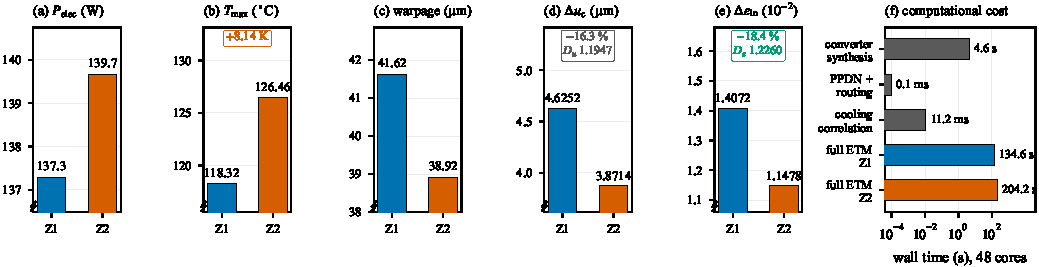
\includegraphics[width=\textwidth]{fig8_final.pdf}
\caption{Historical cross-domain comparison on the frozen repartitioned pair, superseded by the physical lineage of Table~\ref{tab:physical}. The backside
architecture dissipates $2.37$\,W more and runs $8.14$\,K hotter, yet carries a $16.3$\,\%
lower corner-joint displacement driver $\du$ (d) and an $18.4$\,\% lower stabilised local
inelastic response $\Delta\varepsilon_{\mathrm{in}}$ (e). The temperature difference and the
two magnitudes are conditional on the frozen backside representation
(Sec.~\ref{sec:backside-limit}), and the physical lineage of Sec.~\ref{sec:physical} reverses the sign of the driver ordering. The two are distinct quantities: (d)
is a displacement in micrometres and drives the submodel, (e) is the dimensionless per-cycle
response it returns. Warpage is peak-to-valley. Panel (f)
reports the measured cost of one complete evaluation on 48 cores; the thermoelastic and
local solder solves are entered once each, not once per fixed-point iteration. The ordinates
of (a)--(e) are truncated, as the axis break marks.}
\label{fig:final}
\end{figure*}

The results of this subsection are the frozen historical result that motivated the physical closure; they are superseded by the physical lineage of Sec.~\ref{sec:physical} and are retained only to show what the closure changed. Both architectures were frozen on the repartitioned stack before any result was computed, and
one steady-state electrothermal--mechanical solution was obtained for each. The results are
given in Table~\ref{tab:final} and Fig.~\ref{fig:final}.

The backside architecture dissipates $2.37$\,W more, almost entirely because its
through-substrate field carries the 1\,V rail rather than the 48\,V rail, and it runs
$8.14$\,K hotter at the peak---a difference conditional on the backside representation, and
one that changes sign within the bracket of Sec.~\ref{sec:backside-limit}---and its corner
joints run $7.55$\,K hotter than Z1's. It nevertheless carries $18.4$\,\% lower local inelastic response,
$D_{\varepsilon} = 1.2260$, and a $16.3$\,\% lower corner-joint displacement driver,
$D_{u} = 1.1947$. On this pair, ranking the two architectures by peak temperature therefore
gives the opposite answer to ranking them by local mechanical response, which is sufficient
to show that peak temperature is not a reliable proxy for the local mechanical ranking. The
sign of the displacement-driver ordering, unlike that of the temperature difference, is
preserved across every backside representation tested.

The driver and the response order the pair the same way, but they do not agree on magnitude,
and only the second is a measure of solder response. Two cross cases through the same
submodel separate the causes. Applying the backside displacement at the embedded joint
temperature gives $19.39$\,\% below the embedded response, more than the $16.3$\,\%
reduction in the driver itself, because the accumulated inelastic strain depends nonlinearly
on the imposed displacement through \eqref{eq:creep}, whose exponent is about seven at these
temperatures. Applying the embedded displacement at the backside joint temperature raises the
response by $0.75$\,\%. The hotter joint therefore works against the backside architecture
and returns part of its advantage, and the net $18.43$\,\% exceeds the driver separation
despite the temperature, not because of it. Two further quantities returned by the same solve rank the pair
identically: the equivalent inelastic strain range, $1.2257$, and the inelastic work per
cycle, $1.1658$. The stabilised cycle is reached well within the four cycles integrated, the
last two differing by $0.04$\,\% and $0.06$\,\%.

This is not a statement that temperature is unimportant to solder fatigue; temperature-
dependent constitutive behaviour is among the dominant physics in \eqref{eq:creep}. The
narrower and correct statement is that the two rankings are not equivalent, because the local
response is set by the geometry and stiffness distribution of the joint's immediate
neighbourhood as well as by its temperature, and those are architecture properties that peak
temperature does not encode.

\subsection{Realizability status}
Both architectures are geometrically realizable on the repartitioned stack, at a microvia
pitch bounded by reported practice for embedded-die
interconnection~\cite{Ostmann2008ChipEmbedding} and a stacking topology well inside the
qualified configuration for multi-level build-up interconnects~\cite{Cauwe2023HDI}. Neither
is qualified. The microvia current allowable, the capture-pad diameter and a vendor design
rule for the specific build-up technology remain unavailable, as do two package clearance
rules. The status carried forward is therefore \emph{geometrically realizable and
process-conditional}, and the provisioning quantity $n_{\mathrm{req}}$ of \eqref{eq:nreq} is
never presented as a manufacturing requirement.

\subsection{What each physics block contributes}
\begin{table}[!t]
\caption{Contribution of each physics block, same architecture pair, reconstructed
from the successive recorded states of the model. Within each block every row above the
last is a superseded intermediate state of that refinement path, retained to show how
the absolute quantities move; only the final row is a current result.}
\label{tab:ablation}
\centering
\footnotesize
\setlength{\tabcolsep}{2.5pt}
\begin{tabular}{@{}L{2.85cm}cccc@{}}
\toprule
Model state & $P$ (W) & $T_{\max}$ ($^{\circ}$C) & warp (\textmu m) & $\du$ (\textmu m) \\
\midrule
\multicolumn{5}{@{}l}{\emph{Z1 embedded}}\\
Calibrated boundary, lumped VR & $125.10$ & $84.87$ & $20.04$ & $2.745$ \\
+ physical cooling, geometry-derived interconnect, resolved converter & $141.78$ & $123.53$ & $25.37$ & $4.280$ \\
+ corrected materials, architecture-aware spans & --- & --- & --- & $4.645$ \\
+ realizable template, intra-cell interconnect repair & $138.80$ & $118.68$ & $41.70$ & $4.640$ \\
+ conductor-plane topology, repartition & $137.29$ & $118.32$ & $41.62$ & $4.625$ \\
\midrule
\multicolumn{5}{@{}l}{\emph{Z2 backside}}\\
Calibrated boundary, lumped VR & $126.19$ & $83.31$ & $17.24$ & $2.075$ \\
+ physical cooling, geometry-derived interconnect, resolved converter & $143.61$ & $130.31$ & $22.62$ & $3.410$ \\
+ corrected materials, architecture-aware spans & --- & --- & --- & $3.890$ \\
+ realizable template, intra-cell interconnect repair & $141.19$ & $126.91$ & $39.00$ & $3.885$ \\
+ conductor-plane topology, repartition & $139.66$ & $126.46$ & $38.92$ & $3.871$ \\
\midrule
Driver ratio $D_{u}$ & \multicolumn{4}{c}{$1.3225 \!\rightarrow\! 1.2552 \!\rightarrow\! 1.1942 \!\rightarrow\! 1.1943 \!\rightarrow\! 1.1947$} \\
\bottomrule
\end{tabular}
\\[2pt]
{\footnotesize Ratios are formed from the unrounded responses and need not reproduce exactly from the rounded entries.}
\end{table}

Table~\ref{tab:ablation} reports the same architecture pair evaluated as physics is added,
reconstructed from the recorded states of the model. Replacing a calibrated convective
boundary and a lumped regulator with the physical cooling model, the geometry-derived
interconnect and the resolved converter band raises the electronics-scope loss by $13$\,\%
and the peak temperature by $39$\,K, and raises the corner-joint driver by $56$\,\% for the
embedded architecture and $64$\,\% for the backside one. Correcting the package materials and
making the via spans architecture-aware then moves the driver ratio by a further
$-4.9$\,\%, and the interconnect and partition corrections move it by $+0.04$\,\%. Each block
changes the absolute quantities substantially; none changes the ordering.
\section{Discussion and Limitations}\label{sec:discuss}
% BEGIN final-lineage:conditional
\subsection{Architecture preference is conditional}\label{sec:conditional}
The comparison does not produce a universal winner, and the reason is structural rather than
numerical. Moving the converter to the backside changes where the 48\,V enters, so the
electrical comparison becomes a comparison of a package path against an external feed whose
resistance is a design requirement (Sec.~\ref{sec:crossover}). The electrical preference also depends on the electrically minimal through-silicon via field and on a half-density through-silicon via field and on an all-solder attach and on the sparser published attach and on the sparser attach with a column-stiffened card, which change the loss verdict. The mechanical and local preferences depend on what surrounds and cools the converter: under void instead of encapsulated space between the cells, the backside plate behind a thermal interface, a second cold plate under the backside converter and a tenfold lower converter-tier conductivity, at least one mechanical or local verdict moves, because such choices decide which materials expand together. A ranking stated without these neighbouring decisions is therefore not a property of either architecture; the sensitivity matrix of Table~\ref{tab:classb} states which decisions matter.
% END final-lineage:conditional

\subsection{When mechanics matters in DVPD design}
The results support a specific and bounded role for mechanics. It is not established that
mechanics selects a different optimum: no admissible mechanical allowable exists for this
system, so no architecture can be excluded on mechanical grounds. What is established is
that the mechanical response is architecture dependent, that it is not inferable from the
electrical or thermal result, and that it is not captured by global warpage. Mechanics is
therefore design-relevant as a signoff and ranking quantity, and should be evaluated on the
same geometry as the electrical and thermal design rather than afterwards.

\subsection{What is, and is not, a synthesis constraint}
Physical realizability, by contrast, is an active constraint now. A tier order equivalent to
another at the component-selection and stack-budget level can require a via of aspect ratio
$5.05$ (frozen devices; $5.32$ with the selected ones), and the alternative that avoids it
costs nothing in area, height or component count.
Constraints of this kind cannot be discovered by an electrical model, because they depend on
the conductor-plane structure of the package rather than on its netlist; and they cannot be
deferred to a later packaging step, because the remedy is a change of component partition,
which is a synthesis variable.

\subsection{Lateral extent of the backside converter}\label{sec:backside-limit}
% BEGIN final-lineage:backside-limit-frame
This subsection concerns the historical frozen representation (Sec.~\ref{sec:histrep}); the physical architectures of Sec.~\ref{sec:physarch} resolve the lateral structure of the backside converter explicitly.
% END final-lineage:backside-limit-frame
The backside architecture is represented by a converter medium occupying a continuous layer
below the substrate, whereas the embedded architecture carries converter medium only inside
the 49 cell footprints, which cover $30.5$\,\% of the substrate area. The two architectures
therefore do not contain the same volume of converter medium: $1103.40$\,mm$^{3}$ against
$337.02$\,mm$^{3}$, a factor of $3.27$. No source available to this work establishes what
occupies the remaining $69.5$\,\% of the backside, and the question is consequential rather
than cosmetic.

Rerunning the frozen pipeline with that area filled by a non-converter medium, so that both
architectures carry an identical $337.02$\,mm$^{3}$, gives the bracket in
Table~\ref{tab:backside}. The \emph{direction} of the displacement-driver ordering survives
every case. Its magnitude does not: the reduction spans $3.59$--$65.56$\,\%, and the
temperature difference changes sign, from $+8.14$\,K for the frozen representation to
$-2.77$\,K when the out-of-cell area is filled with substrate silicon. The claim that the
backside architecture is the hotter one is therefore \emph{not} established by this work, and
the $16.3$\,\% and $18.4$\,\% figures are reported as conditional on the frozen
representation. The local solder submodel was not rerun across the bracket, so the
$D_{\varepsilon}$ value inherits the same conditionality through $\Delta u_{\mathrm{c}}$ and
the joint temperature.

A physically correct backside would be laterally structured, with cells over part of the area
and the board interface over the rest. The present geometry cannot represent that, because
the ball field is a separate full-area layer below the converter rather than coexisting with
it; resolving it requires a backside construction that no source available to this work
supplies.

\begin{table}[!t]
\caption{Effect of the backside converter's lateral extent on the frozen pair. Z1 is
unaffected. The frozen row reproduces Table~\ref{tab:final} exactly.}
\label{tab:backside}
\centering
\begin{tabular}{@{}lrrr@{}}
\toprule
out-of-cell medium & $T_{\max}$ (\textdegree C) & $\Delta u_{\mathrm{c}}$ (\textmu m) & vs.\ Z1 \\
\midrule
Z1 (reference)                    & $118.32$ & $4.6252$ & --- \\
converter medium (frozen)         & $126.46$ & $3.8714$ & $-16.30$\,\% \\
underfill, $8$\,GPa               & $171.24$ & $1.5930$ & $-65.56$\,\% \\
substrate silicon, $130$\,GPa     & $115.55$ & $4.4591$ & $-3.59$\,\% \\
\bottomrule
\end{tabular}
\end{table}

\subsection{Limitations}
Each limitation below is stated with its effect on the claims.
% BEGIN final-lineage:limit-feed
\emph{The direct feed is specified as a requirement, not as a part.} No connector, cable, bus or
contact resistance for a kilowatt-class direct regulator feed is available to this work; the
construction precedent names connector types only. The platform-inclusive comparison is
therefore stated as a maximum loop resistance, and whether a real feed meets it is not claimed.
The connector drawn in the figures is illustrative.

\emph{The attach is a close analog, not a qualified joint.} Its geometry follows a published
30\,$\mu$m-pitch Cu-pillar process on an organic substrate, and its density is carried between
that construction and a sparser published one; neither is this package's process. Its
current-carrying capability, electromigration margin and fatigue are not evaluated---the
per-bump current density is reported as an output, never against an allowable---its contact
and intermetallic resistance is bounded by the all-solder case, and its mechanical card is
bounded by the underfill-dominated and column-stiffened cards rather than resolved.

\emph{The BGA population is smeared.} The mechanical BGA field is a homogenised layer; the
depopulated field is a uniform scaling of it, and a discrete ball-by-ball depopulation pattern is
not resolved.
% END final-lineage:limit-feed

\emph{Solder constitutive extrapolation.} The creep card is fitted on Sn3.9Ag0.6Cu over
$7.51$--$15.92$\,MPa, whereas $99.8$\,\% of the accumulated inelastic-strain contribution in
this package is generated above that window. The frozen pair is well outside it: the imposed
corner displacement produces an elastic trial shear of $195$ and $159$\,MPa on joints whose
yield stress at temperature is $11.6$ and $10.7$\,MPa, so the joint operates at fifteen to
seventeen times yield and roughly an order of magnitude above the top of the fitted stress
range. The consequence is visible numerically as well as physically: at the tighter
integration tolerance used for the lower-stress cases the time integrator cannot advance at
this operating point at all, while force equilibrium converges to machine zero. This limits
interpretation of the response \emph{magnitude}, which is reported as an envelope. It does
not threaten the ordering: the same ordering is obtained under every constitutive variant
admitted, under all three local metrics returned by the same solves, and under the complete
sequence of geometric corrections in Fig.~\ref{fig:sens}.

\emph{The integration tolerance cannot be bracketed from below.} Of five tolerances evaluated
on the frozen pair, only $5\times10^{-2}$ and $10^{-1}$ admit a solution, and they agree to
twelve digits, so the response is not a product of the tolerance. No tighter tolerance
converges here, so the magnitude is not corroborated against a tight-tolerance reference;
this follows from the stress regime above, not from the integration scheme.

\emph{Absolute life is not computed.} No damage law, life relation or admissible allowable is
established, so no cycles-to-failure and no margin against a requirement is reported. The
paper's claims are ordering and realizability claims and do not depend on absolute life.

\emph{Microvia process parameters are incomplete.} The pitch and stacking topology are
bounded by reported practice, but the diameter, capture-pad geometry, current allowable and a
vendor design rule are unavailable. Consequently neither architecture is described as
manufacturable or qualified; the realizability claim is explicitly conditional and the
provisioning quantity is kept separate from a manufacturing requirement.

\emph{Two package clearance rules remain unsourced.} Their bounds are carried as an envelope
and the realizability verdict is evaluated across it, so the verdict does not depend on a
particular value within that envelope.

\emph{The cooling model is a compact correlation.} A matched conjugate
computational-fluid-dynamics solution of one microchannel half-pitch shows the correlation to be
\ErrCoolingIcepak\,\% conservative in mean base temperature rise at the production load; the
correlation is not recalibrated to it, and the equivalent coefficient is run as a class-B
sensitivity instead. The transitional Reynolds band is refused rather than interpolated.

\emph{Inductor core loss and capacitor dielectric loss are not evaluated.} Only the winding
resistance and the equivalent series resistance are consumed by the loss model. Both
omissions bias the reported dissipation downward and act on the same component set in both
architectures, so the reported ordering is not expected to be altered; exact cancellation is
not claimed, because the two architectures operate at different component temperatures. The
absolute efficiency that may be inferred remains bounded from above.

\emph{Mechanical-to-electrical feedback is neglected.} It is quantified at $0.16$\,\% of the
field resistance in the intact regime, against $22.8$\,\% from the thermal dependence already
inside the fixed point. This justification is specific to the intact regime and does not
extend to a delaminated or cracked interface, which is outside the model.

\emph{Other package failure mechanisms are enumerated but not computed:}
redistribution-layer fracture, delamination, via fatigue, dielectric cracking, pad cratering
and electromigration-assisted damage. The paper makes no claim of completeness over package
failure modes.

\section{Conclusion}\label{sec:concl}

An electrothermal--mechanical framework for distributed vertical power delivery has been
presented in which converter synthesis is propagated into an explicit physical package and
evaluated in one lineage: a conductor-level electrical ledger, a voltage-fed package network on
an aligned graded grid, a tier-aware converged electrothermal fixed point, a thermoelastic package
solution, an all-site critical-joint search and a viscoplastic local submodel. Each reduced model
is checked against a matched reference, and one such check changed a tensor used in every
thermal result.

Physically closing the architectures reveals that no architecture can be ranked independently of its neighboring design decisions: the external feed resistance decides the platform-level electrical preference, through-silicon-via provisioning can reverse the package-internal one, the regulator-to-substrate attach density can change it, cooling and the out-of-cell construction can reverse the mechanical preference, and local construction determines the solder response. A coupled electrothermal--mechanical framework is therefore required to make an architecture-level decision.

The nominal results are reported separately from that conclusion. Inside the package the direct-fed backside regulator dissipates \PlossZtwo\,W against \PlossZone\,W for the embedded one in the continuous-input scenario, an advantage it keeps only while its external 48\,V feed loop stays below \RstarSzero\,m$\Omega$ (\RstarSone\,m$\Omega$ under the buck-duty pulse), a requirement on the feed that no available source shows to be met or missed. Mechanically, the embedded architecture carries the lower die warpage and joint displacement driver in every scenario that admits a valid comparison; thermally,
the embedded architecture runs cooler in the continuous-input scenario, the backside architecture runs cooler in the buck-duty pulse---the peak-temperature ordering reverses with the scenario. Under the overall-ratio pulse the embedded operating point leaves the valid solid-solder domain under the assumed cooling; that scenario is an infeasibility result, and no architecture ordering of any quantity is drawn there. Physical realizability cannot be separated from architecture
selection either: equivalent tier orderings can differ sixfold in worst via aspect ratio, and the
ball count is a solved design variable whose peak loading is not monotone in the count.

All 31 open sensitivity inputs were run on the production mesh or bounded; the electrically minimal through-silicon via field reverses the package-internal loss ordering; void instead of encapsulated space between the cells reverses the joint-driver ordering; a direct-feed loop of 10\,$R^{*}$ (17.7\,m$\Omega$) reverses the platform-inclusive loss ordering; the backside plate behind a thermal interface reverses the peak-temperature, die-warpage and joint-driver orderings; a second cold plate under the backside converter reverses the peak-temperature, die-warpage and joint-driver orderings; a tenfold lower converter-tier conductivity reverses the joint-driver ordering; eleven further inputs only make a resolved ranking unresolved (Sec.~\ref{sec:classb}). The local response is \LocalMeshPhrase{}: its declared mesh family converges for the embedded architecture and is bounded by Richardson extrapolation for the backside one, and a
local ordering is drawn only beyond twice that bound. The results are conditioned on named
input-current scenarios, because the switching schedule of the regulator is not derivable from its
loss model; on an engineering ball-provisioning rule rather than a reliability allowable; on a
direct-feed requirement rather than a specified connector; and on solder response rather than
life. Closing those requires the switch-state schedule of the converter, a characterised direct
feed, a qualified regulator-to-substrate attach of known density, qualified electromigration and
fatigue data for the package metallurgy, and a required life for the application.

\section*{Acknowledgment}
The authors thank the members of the Center for Heterogeneous Integration of Micro Electronic
Systems for discussions on package-level power delivery.

% \balance is disabled: with the present reference list it balances the final two
% columns at the cost of a 2.46 pt overfull vbox on the last page. Re-enable it if the
% reference list changes length.
%\balance
\bibliographystyle{IEEEtran}
\bibliography{ETM_DVPD_REFERENCES}

\end{document}
